\documentclass[journal,10pt]{IEEEtran}
\usepackage[numbers,sort&compress]{natbib}
\input{glyphtounicode}
\pdfgentounicode=1
\usepackage{amsmath,amssymb,amsfonts,mathtools,amsthm,bm}
\usepackage{booktabs,graphicx,array,tabularx,placeins,float,url}
\usepackage[hidelinks]{hyperref}
\hypersetup{pdfauthor={Ali Eslami and Jiangbo Yu}}
\usepackage[protrusion=true,expansion=false]{microtype}
\graphicspath{{figures/}{./}}
\allowdisplaybreaks
\setlength{\emergencystretch}{3em}
\interdisplaylinepenalty=2500
\newtheorem{assumption}{Assumption}
\newtheorem{theorem}{Theorem}
\newtheorem{proposition}{Proposition}
\newtheorem{corollary}{Corollary}
\newtheorem{remark}{Remark}
\newtheorem{definition}{Definition}
\newcommand{\R}{\mathbb{R}}
% elsarticle includes the word ``Appendix'' in appendix-section references.
\newcommand{\appref}[1]{Appendix~\ref{#1}}


\newcommand{\suppnumber}[1]{\csname suppnumber@#1\endcsname}
\newcommand{\suppref}[1]{Supplement~\suppnumber{#1}}
% Cross-document numbers: ordinary definitions; no external auxiliary dependency.
\expandafter\def\csname suppnumber@app:benchmark-details\endcsname{S1.4}
\expandafter\def\csname suppnumber@app:earlier-benchmarks\endcsname{S7}
\expandafter\def\csname suppnumber@app:network-transfer\endcsname{S3}
\expandafter\def\csname suppnumber@app:reusable-benchmark\endcsname{S1}
\expandafter\def\csname suppnumber@app:sequential-handover\endcsname{S1.7}
\expandafter\def\csname suppnumber@app:structure-online-details\endcsname{S2.2}
\expandafter\def\csname suppnumber@app:task-state-protocol\endcsname{S5}
\expandafter\def\csname suppnumber@sec:supp-execution\endcsname{S4}
\expandafter\def\csname suppnumber@tab:new-coordinate-ablation\endcsname{S4}


\begin{document}
\title{Formal Guarantees for Trustworthy Agent-Mediated Urban Perimeter Control}
\author{Ali Eslami and Jiangbo Yu\thanks{The authors are with the Department of Civil Engineering,
McGill University, Montreal, Quebec, Canada (e-mail: ali.eslami@mcgill.ca;
jiangbo.yu@mcgill.ca).}}
\maketitle
\begin{abstract}
Urban perimeter control must manage regional congestion and boundary queues
while satisfying time-specific service obligations. AI agents can support
traffic operators by interpreting evolving network conditions, incidents,
and service priorities and translating them into adaptive control and
replanning requests. However, each new agent-proposed plan must remain
compatible with the evolving traffic state, uncertainty, and outstanding
service obligations. We therefore formulate a runtime certification problem
for agent-proposed perimeter-control plans and develop a
transportation-specific framework that provides formal guarantees of
physical and service feasibility before execution. The framework checks
whether a proposed plan respects vehicle conservation, nonnegative traffic
states, boundary-storage limits, and service deadlines under uncertainty. It
then decides whether the plan can be executed as proposed, should be
modified to restore feasibility, or should be rejected while the previously
accepted plan remains in use, and, when the terminal conditions are
certified, ensures that accepted plans end in a state from which feasible
operation can continue. Numerical studies show that the certificate leaves
feasible plans unchanged, traffic-specific structure reduces conservatism,
and checked repair recovers feasible alternatives. Further experiments show
that the framework can accept beneficial changes while rejecting requests
that would violate boundary-storage or service constraints, including under
computation delays and agent-context errors. Overall, the framework advances
trustworthy AI for transportation systems by providing formal guarantees
that connect adaptive agent decisions to physically and operationally
feasible traffic control.
\end{abstract}
\begin{IEEEkeywords}Agentic AI, Macroscopic fundamental diagram, Perimeter control, Runtime certification, Model predictive control\end{IEEEkeywords}

\section{Introduction}
\label{sec:new-introduction}

Urban perimeter control regulates flows into and between regions as
congestion and external arrivals change. Regional accumulation affects
network traffic production through the macroscopic fundamental diagram
(MFD), which provides a tractable network-scale description of congestion
and trip completion
\cite{daganzo2007gridlock,geroliminis2008existence,daganzo2008analytical,geroliminis2011properties,leclercq2014cross}.
From an operator's perspective, the problem is to regulate regional
accumulation, manage vehicles waiting at region boundaries, and satisfy
time-specific service obligations. These requirements become more difficult
to coordinate when incidents, demand conditions, or operating priorities
change during execution.

Classical MFD perimeter-control methods address regional congestion through
feedback gating and multivariable boundary-flow control
\cite{keyvan2012gating,aboudolas2013perimeter}. Stability analysis and
control-Lyapunov-function designs establish regulation properties under
prescribed traffic dynamics \cite{haddad2012stability,zhong2018robust},
while robust, hybrid, and adaptive formulations extend perimeter regulation
to uncertain observations, switching actions, and changing operating
conditions
\cite{mohajerpoor2020hinf,hajiahmadi2015hybrid,haddad2020adaptive,kouvelas2017adaptive}.

Predictive perimeter control optimizes sequences of gate commands over an
MFD model \cite{geroliminis2013mpc}. Multi-region formulations account for
spatial heterogeneity and route guidance
\cite{ramezani2015heterogeneity,sirmatel2018economic}, while exterior queues
and cordon storage capture the waiting cost and spillback created by
metering \cite{haddad2017queues,ni2019cordon}. State and demand estimation
further support predictive operation when traffic conditions must be
reconstructed from measurements \cite{sirmatel2019estimation}, and recent
MFD calibration work explicitly characterizes loading--recovery variation
and uncertainty \cite{ma2025mfduq}.

AI-based decision tools provide an additional way to adapt perimeter control
as traffic conditions and operator objectives change. Data-driven
perimeter-control methods have used adaptive dynamic programming and
reinforcement learning to learn gating policies from traffic experience
\cite{chen2022dataefficient,chen2024iadp}, while multi-agent approaches
coordinate regional metering, heterogeneous cordon gates, and decentralized
control \cite{zhou2023scalable,yu2025physicsperimeter,li2024beyond}. Related
traffic-signal and language-model studies show how AI systems can generate
actions, interpret contextual information, coordinate decisions, and invoke
external tools
\cite{wei2019presslight,wei2019colight,llmlight2023,masri2025llmtraffic,collmlight2025,trafficgpt2024,openti2024,virtualpolice2026,yu2025statespace}.

These capabilities can support traffic operators when changing network
conditions or service priorities require new control decisions. In this
work, an AI agent serves this higher-level role: it interprets evolving
operating priorities and invokes computational tools, such as numerical
planners, to generate candidate perimeter-control plans.

This added flexibility creates a certification requirement whenever a
proposed plan replaces the plan currently in operation. Each agent-proposed
plan must remain compatible with the traffic state at the time of
activation, uncertainty in that state and future arrivals, available
boundary storage, and any service obligations that are still active.
Evaluation of a newly proposed plan therefore incorporates the traffic state
and outstanding obligations inherited from the operation already under way.
The operator needs a principled way to decide whether the new plan may
replace the current one, whether it should be modified, or whether the
previously accepted plan should remain in operation.

Runtime assurance provides a natural foundation for this decision. Simplex
architectures retain a verified fallback controller
\cite{simplex,mehmood2022black}; control barrier functions and shielding
restrict unsafe actions \cite{ames2017,alshiekh2018}; predictive safety
filters evaluate future constraint satisfaction
\cite{wabersich2021,hsu2023safety}; and runtime-assurance and
reference-governor methods formalize the transfer of control authority
\cite{fisac2019,hobbs2023runtime,gilbert2002generalized,garone2017reference}.
Reachability methods additionally provide tools for propagating uncertainty
over future trajectories \cite{coogan2020mixed,kochdumper2021sparse}. These
methods establish foundations for supervising learning-enabled decisions.
Urban perimeter control also provides structure that can be exploited
directly: vehicles wait at region boundaries for admission to particular
destinations, regional inventories and boundary queues are physically
coupled, and service requirements may remain active across successive
planning requests.

We use this transportation structure to construct a runtime certificate for
agent-proposed perimeter-control plans. The certificate checks whether a
candidate plan satisfies vehicle conservation, nonnegative traffic states,
boundary-storage limits, and time-specific service requirements for all
states and arrivals represented by the uncertainty model. A key observation
is that a vehicle waiting for admission to a destination and the
corresponding destination inventory form a conserved quantity with respect
to that admission flow. Combining these quantities therefore removes the
admission decision from part of the uncertainty propagation. Positivity,
independent queue bounds, and signed uncertainty representations further
tighten the resulting bounds while preserving dependencies in the uncertain
traffic state. Together, these ingredients provide a transportation-specific
representation for checking regional inventories, queues, control inputs,
and service constraints over the planning horizon.

The certificate is then integrated with sequential planning and execution.
If a proposed plan satisfies the required conditions, it can replace the
currently active plan with its commands preserved. A rejected plan enters a
checked repair procedure that searches for a nearby feasible alternative,
with every repaired candidate returned to the same certificate before
execution. If no replacement is accepted, the previously accepted plan
remains active through its certified validity interval. When the terminal
conditions are certified, the framework ensures that accepted plans end in a
state from which feasible operation can continue. It also accounts for
traffic evolution while a new plan is being computed and certified.

The resulting framework provides a formal interface between adaptive
AI-based planning and physical traffic execution. The interface determines
when plans produced by AI models and computational tools are admissible for
the transportation system. The numerical evaluation examines certification
conservatism and checked repair. Further experiments show that the framework
can accept beneficial changes while rejecting requests that would violate
boundary-storage or service constraints, including under computation delays
and agent-context errors.

Therefore, the paper makes four main contributions:
\begin{enumerate}
\item We formulate an execution contract for agentic perimeter control that
connects sequential operator instructions to numerical planning requests while
preserving service requirements, task timing, and plan validity intervals.

\item We develop a structure-preserving nonlinear certification method that
uses class--queue incidence, positivity, and signed uncertainty propagation to
verify continuous physical constraints and scheduled service requirements.
The method extends to networks with several exterior queues. A replacement
theorem carries these guarantees through successive replanning and continued
execution after rejection, while a terminal-backup result gives sufficient
conditions for certified continuation beyond finite-plan expiry.

\item We formulate a certification-aware predictive filter over a finite
family of backup interpolations. We prove availability and minimum intervention
relative to the tested grid, preserve certified execution on timeout, and
give terminal conditions for certified continuation beyond finite-plan expiry.

\item We specify a reusable family of regional-regulation, queue-economic and deadline-constrained replanning tasks. Matched CLF, predictive and physical-CBF implementations separate controller performance from physical, service and family-certification outcomes. A complete deadline grid, checked reserve refresh, delayed-handover test, connected-network study and actual live agent-to-planner traces quantify the operational consequences of execution authority.
\end{enumerate}

Section~\ref{sec:new-problem} formulates the traffic-control problem. Section~\ref{sec:new-agent} defines the agent and planning interface, and Section~\ref{sec:new-certification} develops plan certification and execution. Section~\ref{sec:new-evidence} evaluates the method; Section~\ref{sec:new-discussion} discusses operational implications. Detailed proofs and numerical specifications appear in the appendices and supplement.

\begin{table*}[!t]
\centering\small
\caption{Principal notation. Traffic inventories are expressed in units of
100 vehicles unless a table states physical vehicles.}
\label{tab:nomenclature}
\begin{tabular}{@{}p{0.20\linewidth}p{0.72\linewidth}@{}}
\toprule
Symbol & Meaning\\
\midrule
$n_i$, $n_{ij}$ & Regional accumulation; vehicles in region $i$ destined for $j$\\
$z$, $x$, $M$ & Exterior waiting inventory; physical state; total vehicle inventory\\
$u_{ij}$, $a$ & Fractional gate command; realized exterior admission flow\\
$\Lambda$, $d_{ij}$ & Exterior arrivals; destination-specific internal demand\\
$d$, $\bar w_{\rm veh}$ & Sensing half-width (vehicles); physical arrival-residual bound (vehicles/h)\\
$\bar w_x$ & Normalized arrival-residual bound $\bar w_{\rm veh}/100$ (inventory units/h)\\
$\mathcal S_t$ & Decision record: state set, uncertainty, task, active plan, time and versions\\
$P$, $P^B$, $\mu_B$ & Proposed plan; verified continuation; terminal backup policy\\
$P_a$, $c$ & Destination-allocation matrix; network destination-class vector\\
$t_f$, $\eta$ & Example service deadline and inventory limit\\
$T_r$, $g_r$, $\eta_r$ & General service time, row vector and threshold\\
$\theta_i$, $\vartheta$ & Agent task record; predictive-repair interpolation weight\\
$K_b$, $K$, $\mathcal K$ & Feedback gain; local block count; terminal invariant set\\
$\beta_j^{\rm phys}$, $b_a$ & Physical constraint-row limit; admission-incidence vector\\
$y$, $L$ & Conservation-coordinate state and its invertible transform\\
$r_l$, $R_l$ & Starting and trial-tube radii on interval $l$\\
$a_{il}$, $b_{ijl}$ & Local diagonal and off-diagonal Jacobian bounds\\
$\xi$, $\Gamma_l$, $\zeta_l$ & Initial uncertainty, signed generator and nonlinear remainder\\
$z_e$ & Prediction-error coordinate used only in the enclosure proof\\
$J_R$, $J_Q$, $J_D$ & Native regulation, queue-economic and weighted-priority objectives\\
$p$, $E$, $x^R$ & Regional-priority weight; finite-plan endpoint; native four-state vector\\
$\mathcal C$, $\mathcal F_{\mathcal C}$, $\widehat{\mathcal F}_{\mathcal C}$ & Planning contract; robust feasible and checker-certified plan sets\\
$X_i^A$, $h_i$, $\iota_i$ & Agent interface state, memory and supplied contextual view\\
$J_2$, $\varrho_r$ & Earlier Region-2 priority cost and retained-benefit fraction\\
$\mathrm{TTS}$ & Total time spent, including vehicles waiting outside\\
\bottomrule
\end{tabular}
\end{table*}

\FloatBarrier
\section{Two-Region MFD Perimeter-Control Problem}
\label{sec:new-problem}
Here, we use a two-region network as the primary setting because it is the smallest
configuration that captures interregional transfers, destination-specific
vehicle classes, exterior admission, and regional service requirements while
keeping the certification construction transparent. The model also follows
established two-region MFD perimeter-control formulations. Section~\ref{sec:network-extension}
extends the certification construction to networks with multiple regions and
exterior queues.


\subsection{Traffic inventories, destination flows and boundary storage}

The physical state comprises the total vehicle accumulation in each region, destination-specific vehicle classes, and an exterior staging reservoir:
\begin{equation}
\begin{aligned}
x&=(n_1,n_2,n_{11},n_{22},n_{10},n_{20},z)^\top,\\
u&=(u_{12},u_{21},u_{02},u_{20})^\top.
\end{aligned}
\label{eq:new-state}
\end{equation}
Here $n_i$ denotes the total vehicle accumulation in region $i$, with
$i\in\{1,2\}$. The variable $n_{ij}$ counts vehicles currently in region
$i$ whose destination is $j$, where $j\in\{0,1,2\}$ and $j=0$ denotes the
exterior. Thus, $n_{ii}$ represents vehicles that complete their trips
within region $i$, $n_{12}$ and $n_{21}$ represent interregional traffic,
and $n_{10}$ and $n_{20}$ represent vehicles destined for the exterior.

Exterior-destined vehicles in Region~1 leave the network through Region~2.
Because the destination classes within each region sum to the regional total,
the interregional class inventories are recovered from the regional totals
and stored classes as
\[
n_{12}=n_1-n_{11}-n_{10}, \qquad
n_{21}=n_2-n_{22}-n_{20}.
\]
The separate queue $z$ represents vehicles waiting outside the controlled
regions for admission. One state unit represents 100 vehicles, and time is
measured in hours. Inventories are continuous aggregate quantities, and
their evolution is described by continuous-time differential equations.
The variables $n_{ij}$ describe stored vehicle inventories; $q_{ij}$ below
describes their potential outflow rate in inventory units/h.

Following the two-region perimeter-control models in
\cite{zhong2018robust,geroliminis2013mpc}, we use the cubic MFD
\begin{equation}
\begin{aligned}
G(n)&=0.0014877n^3-0.29815n^2+15.0912n,\\
q_{ij}&=n_{ij}v(n_i),
\end{aligned}
\label{eq:new-mfd}
\end{equation}
where
$v(n)=0.0014877n^2-0.29815n+15.0912$
equals $G(n)/n$ for $n>0$ and is defined by continuity at $n=0$. The potential class outflow $q_{ij}$ is defined
before gating. The aggregate rate $G(n_i)$ describes potential trip
completion and transfer out of region $i$, allocated among destination
classes in proportion to their inventories. This MFD has a critical accumulation of 3391.93 vehicles
and a peak potential outflow of 6.303 vehicles/s. We impose an operational upper bound of 10,000 vehicles per region; this bound is a model constraint at which the fitted MFD retains positive production. Class flows assume comparable within-region trip
lengths, destination-proportional mixing, and adequate receiving supply
throughout the verified domain.

Exterior arrivals are $\Lambda(t)=\widehat\Lambda(t)+w(t)$, with specified
forecast $\widehat\Lambda$ and bounded measurable residual $w$.
For destination fraction $\pi=1/2$ toward Region~1,
\begin{equation}
a(z,u_{02})=\min\{60z,120u_{02}\},\qquad
\dot z=\Lambda-a.
\label{eq:new-admission}
\end{equation}
These branches represent a one-minute staging release time and commanded
admission capacity. The queue explicitly accounts for boundary storage
\cite{haddad2017queues}; its limit measures aggregate overflow. Spatial
spillback requires a receiving-supply extension.

The gate commands are dimensionless fractions. Interregional and exit
commands multiply the corresponding potential class flows; $u_{ij}=1$
permits the full potential flow and $u_{ij}=0$ blocks it. Exterior
admission instead follows \eqref{eq:new-admission}, with $u_{02}$ scaling
the admission capacity. Commands may vary over time or be held on finite
planning blocks. They represent aggregate boundary-flow allocations.
For a class with potential flow $q$ and associated gate fraction $u_g$,
the physical number transferred over $[t_a,t_b]$ is
$100\int_{t_a}^{t_b}u_g(t)q(t)\,dt$.

With fixed primitive demands and sums
$d_1=d_{11}+d_{12}+d_{10}$, $d_2=d_{22}+d_{21}+d_{20}$, conservation gives
\begin{equation}
\begin{aligned}
\dot n_1&=-q_{11}-(q_{12}+q_{10})u_{12}+q_{21}u_{21}+d_1,\\
\dot n_2&=-q_{22}+(q_{12}+q_{10})u_{12}-q_{21}u_{21}
                 +a-q_{20}u_{20}+d_2,\\
\dot n_{11}&=-q_{11}+q_{21}u_{21}+d_{11},\\
\dot n_{22}&=-q_{22}+q_{12}u_{12}+(1-\pi)a+d_{22},\\
\dot n_{10}&=-q_{10}u_{12}+d_{10},\\
\dot n_{20}&=-q_{20}u_{20}+q_{10}u_{12}+d_{20},\\
\dot z&=\widehat\Lambda+w-a.
\end{aligned}
\label{eq:new-plant}
\end{equation}
A transfer preserves a vehicle's destination while changing its current
region. For example, a vehicle transferred from class $n_{21}$ enters
$n_{11}$, which is already included in $n_1$; its trip subsequently
completes at the local outflow rate $q_{11}$. Command changes preserve
physical inventories, which remain continuous across planning blocks.
The gate fractions satisfy
\begin{equation}
\mathcal U=\{u:0\le u\le1,\ |u_{21}-u_{12}|\le0.75,
\ |u_{20}-u_{02}|\le0.75\}.
\label{eq:new-gates}
\end{equation}
The six classes are nonnegative, $0\le n_1,n_2\le100$, and $0\le z\le20$.
Together with \eqref{eq:new-gates}, these give 24 affine state--command
inequalities, checked directly using the plan commands and unmodified
inventory values.
The initial state is $(30,30,15,15,5,5,2)$ and base exterior arrivals are
6000 vehicles/h. Internal demands are constructed once from this operating
record and held fixed across targets and policies
(\appref{app:new-model}).

\subsection{Service obligations and queue-inclusive performance}

The operator specifies service through scheduled affine rows
$g^\top x(t_f)\le\eta$, which can express a regional clearance target or an
imbalance band. For example, the original incident grid uses
\begin{equation}
100n_1(t_f)\le2850\ \text{vehicles},\qquad t_f=1\ \text{h}.
\label{eq:new-service}
\end{equation}
This requirement must hold at the specified deadline \(t_f\), even if the regional accumulation falls below the target earlier. The planner may change its control reference or soft optimization objective, but the authorized service target and its deadline can be changed only by the operator. The binding-service experiment uses 1700 vehicles
at the same deadline.

The planner minimizes queue-inclusive total time spent (TTS). Adding the regional and exterior-queue balances cancels internal transfers and admission flows, so the total inventory changes only through external arrivals, internal demand, and completed departures:
\begin{equation}
\begin{aligned}
M&=n_1+n_2+z,\\
\dot M&=d_1+d_2+\Lambda-F_{\rm out},\\
F_{\rm out}&=q_{11}+q_{22}+q_{20}u_{20},\\
\mathrm{TTS}&=100\int_0^{T_{\rm eval}} M(t)\,dt.
\end{aligned}
\label{eq:new-conservation}
\end{equation}
Here $T_{\rm eval}$ denotes the evaluation horizon. Queue time
$100\int_0^{T_{\rm eval}} z\,dt$ is already included. Completed departures
$100\int_0^{T_{\rm eval}} F_{\rm out}\,dt$ differ from potential MFD outflow,
which also counts transfers before gating. For matched arrivals and initial
inventory, departure differences equal
$-100\Delta M(T_{\rm eval})$. Counting waiting vehicles
therefore makes the resource cost of restricting admission explicit.

\subsection{A reusable family of perimeter-control tasks}
\label{sec:benchmark-formulation}

We distinguish three tasks according to the transportation decision being
evaluated. Each task fixes the dynamics, available information, command limits,
initial condition and evaluation interval before comparing methods.

\paragraph{R: regional regulation}
The native two-gate formulation of \cite{zhong2018robust} uses four
destination classes $x^R=(n_{11},n_{12},n_{21},n_{22})^\top$ and regional
totals $n_1=n_{11}+n_{12}$, $n_2=n_{21}+n_{22}$. With the class flows in
\eqref{eq:new-mfd}, its balances are
\begin{equation}
\begin{aligned}
\dot n_{11}&=d_{11}-q_{11}+u_{21}q_{21},\\
\dot n_{12}&=d_{12}-u_{12}q_{12},\\
\dot n_{21}&=d_{21}-u_{21}q_{21},\\
\dot n_{22}&=d_{22}-q_{22}+u_{12}q_{12}.
\end{aligned}
\label{eq:benchmark-native}
\end{equation}
The task regulates both totals to $n_i^\star=30$ while maintaining
nonnegative classes, regional storage and the specified two-gate intervals.
We evaluate
\begin{equation}
J_R=10^4\int_0^{3/2}\bigl[(n_1-30)^2+(n_2-30)^2\bigr]\,dt.
\label{eq:benchmark-regulation-cost}
\end{equation}
Its units are veh$^2$-h. This native regulation task supplies a direct
comparison with the reproduced almost-smooth CLF law. The queue-aware tasks
below additionally require the admission and exit channels of
\eqref{eq:new-plant}.

\paragraph{Q: queue-inclusive economic planning}
At $t_0=1/3$ h, use the seven-state information set $\mathcal I_{t_0}$,
arrival forecast and bounded residual of \eqref{eq:new-plant}. A numerical
planner requests two constant gate blocks through the absolute endpoint
$E=1$ h. Subject to the physical rows, the objective is
\begin{equation}
J_Q(P)=100\int_{t_0}^{E}(n_1+n_2+z)\,dt.
\label{eq:benchmark-queue-cost}
\end{equation}
Exterior arrivals continue to join the queue when admission is restricted.
Thus $J_Q$ measures the traffic consequence of metering, including waiting
outside the controlled regions \cite{haddad2017queues}. The predictive tool
follows the MFD planning approach of \cite{geroliminis2013mpc} with the
explicit model, blocking and objective supplied here.

\paragraph{D: deadline-constrained plan replacement}
The same plant and information are supplemented by
$100n_1(E)\le\eta$ vehicles and a soft Region-2 priority with weight
$p\ge1$. The requested objective is
\begin{equation}
J_D(P)=100\int_{t_0}^{E}(n_1+p n_2+z)\,dt.
\label{eq:benchmark-priority-cost}
\end{equation}
For a physical sensing half-width $d$ vehicles and arrival-residual bound
$\bar w_{\rm veh}$ vehicles/h, define the normalized bound
$\bar w_x=\bar w_{\rm veh}/100$ in inventory units/h. The uncertainty
contract is
\begin{equation}
\begin{aligned}
\mathcal I_{t_0}&=\widehat x_{t_0}+[-d/100,d/100]^7,\\
|w(t)|&\le\bar w_x,\qquad t\in[t_0,E].
\end{aligned}
\label{eq:benchmark-contract}
\end{equation}
\paragraph{Feasible plans and certifiable plans}
For Tasks Q and D, collect the information set, uncertainty family, model,
physical rows, scheduled service rows and absolute interval $[t_0,E]$ in a
contract $\mathcal C$. The plan class consists of the executable finite
schedules defined in Section~\ref{sec:new-agent}. Write
$x_P(s;x_0,w)$ for their traffic trajectories. The robust feasible set is
\begin{equation}
\begin{aligned}
\mathcal F_{\mathcal C}=\{P:\;&\forall x_0\in\mathcal I_{t_0},\ w\in\mathcal W,\\
&H_jx_P(s;x_0,w)+J_ju_P(s;x_0,w)
                         \le\beta_j^{\rm phys}\\
&\hspace{1em}\text{for all }s\in[t_0,E]\text{ and physical rows }j;\\
&g_r^\top x_P(T_r;x_0,w)\le\eta_r
\quad\text{for all service rows }r\}.
\end{aligned}
\label{eq:benchmark-feasible-set}
\end{equation}
Here $\mathcal W$ contains all measurable residuals satisfying the stated
bound, and each service time $T_r$ lies in $[t_0,E]$. Membership also
requires a well-defined trajectory throughout that interval. Task Q has
an empty service-row collection; Task D includes the minute-60 regional
row. The sound checker constructs a computable inner set
\begin{equation}
\widehat{\mathcal F}_{\mathcal C}
=\{P:\mathsf C_{t_0}(P\mid\mathcal C)=1\}
\subseteq\mathcal F_{\mathcal C}.
\label{eq:benchmark-certifiable-set}
\end{equation}
The containment follows from the enclosure and execution results in
Section~\ref{sec:new-certification}.

The costs in \eqref{eq:benchmark-queue-cost} and
\eqref{eq:benchmark-priority-cost} depend on the initial state and residual;
we write these arguments explicitly as $J_Q(P;x_0,w)$ or $J_D(P;x_0,w)$
when comparing realizations. In the experiments, a planner minimizes a
center-forecast cost subject to its nominal or finite-scenario constraints.
Execution then selects a certified output for the same contract, using
the center-forecast cost to compare available certified tools. This
distinguishes the numerical planning objective from the robust feasibility
requirement. The local optimizers supply candidates and reported objective
values; the checker supplies their continuous uncertainty-family coverage.

An incumbent already certified for this task continues until a replacement
passes its activation-time check. A reserve synthesized for a changed
uncertainty contract receives a fresh certificate before becoming an
authorized endpoint for repair. Passing a finite realization set records
performance on that set; an exhibited violation identifies an infeasible
member of the uncertainty family. Acceptance by the checker establishes
the physical and scheduled-service properties for the entire family.

For each task, results identify the numerical information received by each
method, the tested realization set and the properties established by its
certificate. This specification lets another planner, estimator or execution
supervisor reuse the same transportation problem and report its performance
and validity domain together.

\section{Agent-Mediated Planning and Execution Authority}
\label{sec:new-agent}

The agent converts changing operator instructions into planning requests.
Numerical tools produce candidate gate schedules, and the execution layer
checks their inherited traffic and service requirements.

\subsection{Sequential information and planning requests}

At proposal time $t_i$, memory $h_i$, task record $\theta_i$ and input $o_i$
(observation and instruction) form the interface state:
\begin{equation}
\begin{aligned}
X_i^A&=(h_i,\theta_i,o_i),\\
\iota_i&=\mathsf{View}(o_i,\theta_i),\\
r_i^A&\sim\Pi_\phi(\cdot\mid h_i,\iota_i),\\
(\theta_i^+,q_i^A)&=\mathsf{Compile}_{t_i}(\theta_i,r_i^A),\\
\mathcal P_i^{\rm prop}
&=\mathsf{Planner}(q_i^A,\mathcal I_i,\mathcal T_i),\\
(u_i^{\rm exec},\ell_i)
&=\mathsf{CertifyExecute}(\mathcal P_i^{\rm prop},s_i),\\
\theta_{i+1}&=\mathsf{Age}_{t_{i+1}}(\theta_i^+),\\
h_{i+1}&\sim\mathsf U_\phi(\cdot\mid
h_i,\iota_i,r_i^A,u_i^{\rm exec},\ell_i,o_{i+1}).
\end{aligned}
\label{eq:new-agent-state}
\end{equation}
A history-only view supplies the observation and memory; a task-record view
also supplies the active priority and its absolute expiry. The trained model
$\Pi_\phi$ proposes an operation, and the compiler checks its fields and
transition before forming $q_i^A$. The record stores active and suspended
priorities with their original expiries. Set, interrupt, continue, extend,
resume and cancel operations, together with $\mathsf{Age}_t$, govern their
evolution. Aging applies before compilation and between proposals, restoring
the latest unexpired predecessor or the default network objective. Invalid
operations leave the time-updated record in place and generate no new request.
\appref{app:task-state-compiler} gives the transitions and temporal invariant.

The resulting priority and duration set the planner's soft objective.
Physical information $\mathcal I_i$ and authorized service requirements
$\mathcal T_i$ remain separate inputs. Thus a schema-valid request can
change the objective even while execution retains an older certified plan.
Interpretation accuracy is scored at the compiled request; physical and
service guarantees concern the executed plan. Memory update $\mathsf U_\phi$
uses the request, executed command, certification feedback $\ell_i$ and next
observation. Singleton memory gives the memoryless special case.

MPC and feedback-rollout tools supply numerical plans. After rejection, the
optional predictive repair tool supplies a modification or a no-result status:
\begin{equation}
\widehat P_i^R=\mathsf{RepairTool}(P_i^0,P_i^B,s_i,\Theta).
\label{eq:repair-tool-interface}
\end{equation}
The decision record $s_i:=\mathcal S_{t_i}$ contains physical information,
absolute time, model and constraint versions, authorized obligations and the
active verified continuation. Every tool output passes the same checker.
An accepted plan replaces that continuation; rejection retains its original
schedule and expiry. Section~\ref{sec:predictive-repair} supplies the repair
and installation rules, including preparation for a future activation slot.

\begin{figure*}[t]
\centering
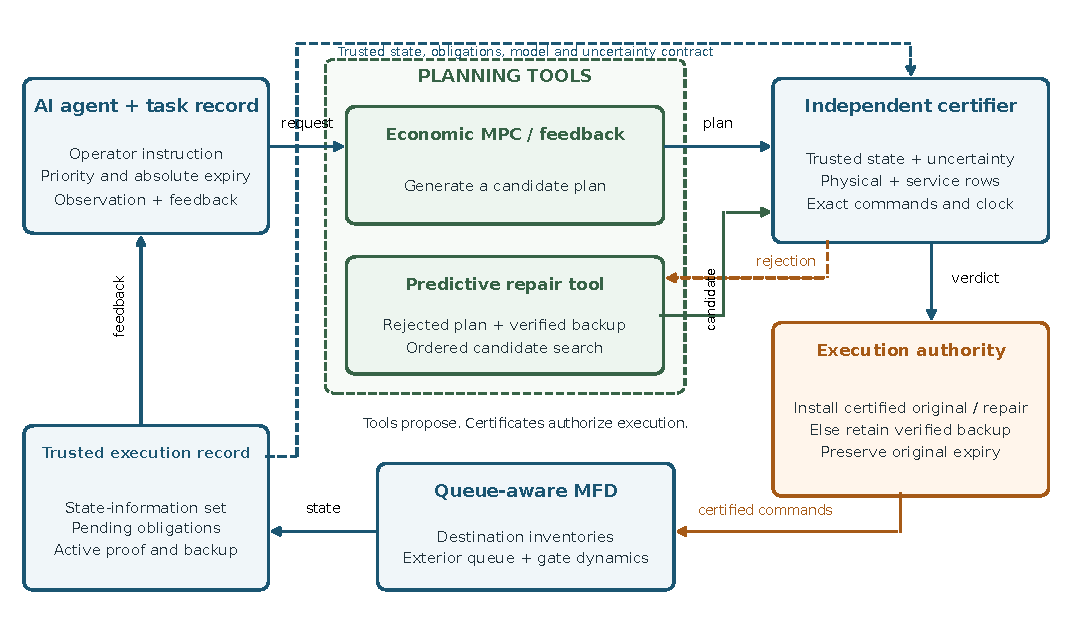
\includegraphics[width=0.98\textwidth]{figures/mfd_tool_architecture.pdf}
\caption{Agent interpretation, numerical planning and execution authority.
MPC, feedback rollout and predictive repair submit candidates to the same
certifier. Execution uses an accepted plan or the still-valid continuation;
the certified terminal policy supplies the expiry transition when available.
Memory and retrieved context affect requests, while the physical state,
obligations and uncertainty contract determine admission.}
\label{fig:new-architecture}
\end{figure*}

\subsection{Executable plans and validity intervals}

A finite plan specifies command blocks $u=k_b+K_bx$ on absolute intervals.
Target-centered feedback has $k_b=u_b^\star-K_bx_b^\star$; constant MPC
commands use $K_b=0$. An accepted replacement begins at its certified
installation time. Rejection preserves the unexecuted schedule, including
already authorized command changes, through its original expiry.
Proposal epochs, replacements and physical command changes are distinct:
a replacement can preserve its first command, and a rejected request changes
none. The decision grid is locally finite. The terminal construction in
\appref{sec:terminal-backup} supplies conditions for continuation beyond expiry.

\section{Structure-Preserving Runtime Certification}
\label{sec:new-certification}

Authorizing a perimeter-control plan requires following the vehicles already
inside the regions together with those waiting for admission. Their
destination classes determine which regional inventories receive the waiting
vehicles. The certificate preserves this relationship while propagating
uncertainty and checking storage, command and service requirements over the
plan's full validity interval.

To construct the certification enclosure, we introduce the transformed state
\begin{equation}
\begin{aligned}
y=Lx=(&n_{11},n_{12},n_{10},n_{22}+(1-\pi)z,\\
      &n_{21}+\pi z,n_{20},z)^\top.
\end{aligned}
\label{eq:new-conservation-coordinates}
\end{equation}
The transformation combines each destination class that receives admitted
vehicles with the corresponding share of the exterior queue. As a result, the
admission flow cancels from the dynamics of these combined inventories and
remains explicitly only in the queue equation. This preserves the relevant
vehicle-conservation relationships during uncertainty propagation and reduces
conservatism in the certification analysis. The first six components of $y$
sum to the total system inventory $M=n_1+n_2+z$. The following construction
uses these coordinates to enclose each proposed plan and then carries the
resulting guarantees through sequential plan replacement and continued
execution after rejection.

\subsection{Plans, uncertainty, and transportation constraints}

A plan beginning at time $t_0$ consists of finitely many command blocks on
$[t_0,E]$, where $E$ is its absolute expiry. The residual bound $\bar w_x$ uses
the normalized flow units defined in Section~\ref{sec:benchmark-formulation}.
On block $b$, write
\begin{equation}
 u_b(x)=k_b+K_bx,
 \qquad \Lambda(t)=\widehat\Lambda(t)+w(t),
 \qquad |w(t)|\le\bar w_x.
 \label{eq:new-plan-data}
\end{equation}
In the primary two-region construction, the forecast $\widehat\Lambda$ is
continuous and piecewise affine, and $w$ is any measurable signal satisfying
the bound. Target feedback uses
$k_b=u_b^\star-K_bx_b^\star$; constant MPC commands use $K_b=0$.
Furthermore, command changes preserve physical inventories.

The trusted physical contract is a finite set of affine rows
\begin{equation}
 H_jx+J_ju\le \beta_j^{\rm phys},
 \qquad j=1,\ldots,n_c.
 \label{eq:new-physical-rows}
\end{equation}
These include nonnegative destination classes, regional and exterior storage,
gate boxes, and paired-gate differences. On block $b$ the row is
$h_{jb}^{\top}x\le\beta_{jb}$, with
$h_{jb}^{\top}=H_j+J_jK_b$ and $\beta_{jb}=\beta_j^{\rm phys}-J_jk_b$.
An operator service task consists of scheduled affine requirements
\begin{equation}
 g_r^{\top}x(T_r)\le\eta_r,
 \qquad r=1,\ldots,n_s.
 \label{eq:new-service-rows}
\end{equation}
Write $e_i$ for the $i$th standard coordinate vector. The Region~1 incident
deadline uses $g_r=100e_1$ and $\eta_r=2850$ vehicles
in the normalized state coordinates. A two-sided regional imbalance band is
represented by two rows. The operator fixes these rows, deadlines, and their
task version; they remain unchanged by the agent's memory or proposals.

\subsection{A computable enclosure that retains conservation structure}

Let $y=Lx$ be the invertible destination-class transformation in
\eqref{eq:new-conservation-coordinates}. If $b_a$ is the incidence vector of
admission in the physical balances, it satisfies
\begin{equation}
 Lb_a=-e_7,
 \qquad Le_7=(0,0,0,1-\pi,\pi,0,1)^\top.
 \label{eq:new-conservation-incidence}
\end{equation}
Admission cancels from the two combined inventories, leaving its nonsmooth
minimum explicitly only in the queue equation. Regional production retains
its dependence on the full transformed state.

For a fixed block, denote the physical field under its nominal forecast by
$f_b(x,t)$. The actual field is $f_b(x,t)+e_7w(t)$. Partition the plan at
command changes, forecast knots, service times, and prediction checkpoints.
On one interval $[t_l,t_l+h_l]$, choose a differentiable predictor $p_l(t)$
and inherited componentwise radii $r_l\ge0$ such that
$|L(x(t_l)-p_l(t_l))|\le r_l$. The implementation uses quadratic predictors.
For candidate outer radii $R_l>0$, construct bounds on
$p_l(t)+L^{-1}[-R_l,R_l]$:
\begin{equation}
 \begin{aligned}
 a_{il}&\ge\sup (L D_xf_b L^{-1})_{ii},\\
 b_{ijl}&\ge\sup |(L D_xf_b L^{-1})_{ij}|\quad(j\ne i),\\
 \delta_{il}&\ge\sup_t |(L f_b(p_l(t),t)-L\dot p_l(t))_i|.
 \end{aligned}
 \label{eq:new-local-bounds}
\end{equation}
At an admission-branch boundary the Jacobian bounds include the convex hull
of both branch Jacobians. Verified exclusion of a branch throughout the
outer tube permits its removal from the bound. The diagonal bound $a_{il}$
retains its sign; cross-component effects enter through magnitudes.

Define the nonnegative forcing and its scalar comparison solution by
\begin{align}
 c_{il}(R_l)&=\sum_{j\ne i}b_{ijl}R_{jl}
                 +\delta_{il}+|(Le_7)_i|\bar w_x,\nonumber\\
 \phi_{il}(s)&=e^{a_{il}s}r_{il}
                  +\chi(a_{il},s)c_{il}(R_l),\nonumber\\
 \chi(a,s)&=\begin{cases}(e^{as}-1)/a,&a\ne0,\\s,&a=0.\end{cases}
 \label{eq:new-component-comparison}
\end{align}
The interval passes its enclosure test when
\begin{equation}
 \max\{r_{il},\phi_{il}(h_l)\}<R_{il}
 \qquad\text{for every }i.
 \label{eq:new-self-inclusion}
\end{equation}
Continuous physical admissibility is verified by the row supports
\begin{equation}
 \sup_{t\in[t_l,t_l+h_l]}h_{jb}^{\top}p_l(t)
             +|h_{jb}^{\top}L^{-1}|R_l\le\beta_{jb}.
 \label{eq:new-affine-support}
\end{equation}
Absolute values of vectors and matrices are componentwise. If the next
predictor recenters by an amount bounded by $\omega_l\ge0$ in $L$ coordinates,
propagate $r_{i,l+1}=\phi_{il}(h_l)+\omega_{il}$. At a service checkpoint,
the resulting center $\widehat x(T_r)$ and radius $r(T_r)$ give the test
\begin{equation}
 g_r^{\top}\widehat x(T_r)+|g_r^{\top}L^{-1}|r(T_r)\le\eta_r.
 \label{eq:new-service-support}
\end{equation}

\begin{theorem}
\label{thm:new-plan-enclosure}
Consider the MFD field \eqref{eq:new-plant} with admission
\eqref{eq:new-admission}, a finite affine-command plan, and the uncertainty
class \eqref{eq:new-plan-data}. Let its initial information set be contained
in the initial predictor box. Suppose the bounds
\eqref{eq:new-local-bounds} are sound and
\eqref{eq:new-self-inclusion} holds on every interval. Then the propagated
boxes contain every trajectory from that initial set under every allowed
residual. If \eqref{eq:new-affine-support} and
\eqref{eq:new-service-support} also pass, the trajectory satisfies every
physical row continuously through the plan's expiry and every included
service row at its deadline. At command or target changes, the inherited box
is propagated and the successor command rows are checked on that box.
\end{theorem}

\begin{proof}
Before a first hypothetical exit from an outer box, the transformed error
magnitude in component $i$ satisfies the scalar differential inequality
\[
\dot v_i\le a_{il}v_i+c_{il}(R_l)
\]
almost everywhere. Its comparison solution is given by
\eqref{eq:new-component-comparison}. Since this solution is monotone over the
interval, the self-inclusion condition
\eqref{eq:new-self-inclusion} rules out a first exit. Hence, every admissible
trajectory remains inside the enclosure throughout the interval.

At the interval endpoint, the error relative to the current predictor is
bounded by $\phi_{il}(h_l)$. If the predictor is recentered for the next
interval, the center shift is bounded by $\omega_{il}$. Because the physical
state is continuous across command or target changes, the same state is
inherited by the next interval. The triangle inequality therefore gives
\[
r_{i,l+1}=\phi_{il}(h_l)+\omega_{il},
\]
which ensures that the successor box also contains every admissible inherited
state.

Applying this argument inductively over the finite partition yields
containment over the full plan horizon. The affine support conditions
\eqref{eq:new-affine-support} and \eqref{eq:new-service-support} then imply
that the physical constraints hold continuously and that the scheduled
service requirements are satisfied at their respective deadlines. The
complete nonsmooth argument and numerical verification rules are given in
\appref{app:new-enclosure-proof}.
\end{proof}

This enclosure checks a plan against the actual forecast and its residual
allowance, including forecast--design mismatch. Target changes carry physical
uncertainty forward, while constant actuator rows are checked exactly. The
result supplies both continuous storage and gate checks and the regional
inventory bound at each service deadline.

\subsection{Positivity, queue comparison, and retained correlations}
\label{sec:structure-certificate}

The general enclosure developed above can be tightened by exploiting additional
structure of the traffic model. Each regional total equals the sum of its
destination-class inventories. Preserving these relationships supplies valid
information that can tighten the certification bounds.

Two useful properties follow directly from the traffic balances. First, if the
destination-class demands, offered arrivals, and constant commands are
nonnegative, then all six destination inventories and the exterior queue remain
nonnegative. For the polynomial completion factor used here,
$v(n)=G(n)/n$ is positive over the relevant domain, while conservation bounds
the total number of vehicles by the initial inventory together with cumulative
offered inflow. Thus, nonnegativity can be established independently of the
upper regional and queue-storage constraints.

Second, under a constant admission command, the queue dynamics are independent
of the regional states:
\begin{equation}
 \dot z=\widehat\Lambda(t)+w(t)-\min\{60z,120u_{02}\}.
 \label{eq:structure-scalar-queue}
\end{equation}
A scalar comparison argument therefore provides continuous lower and upper
bounds on $z$ from the extreme initial queue values and admissible arrival
bounds. Positivity directly verifies the lower bounds on the destination
classes and queue, while the scalar comparison checks the exterior-storage
constraint independently of the full state enclosure. Intersecting these
independently valid bounds with the propagated endpoint enclosure, and then
enclosing the intersection by an outward-rounded box, gives a first
refinement for the next propagation interval.

A second refinement propagates initial-state uncertainty through signed
generators, preserving dependencies among state components throughout the plan. On predictor interval $l$, write
\begin{equation}
 \begin{aligned}
 L(x-p_l)&=\Gamma_l(s)\xi+\zeta_l(s),\qquad |\xi|\le\mathbf1,\\
 \Gamma_l(s)&=e^{A_l^0s}\Gamma_l(0),\qquad |\zeta_l(0)|\le\rho_l.
 \end{aligned}
 \label{eq:structure-affine-set}
\end{equation}
Here, $\xi$ represents the common initial uncertainty, $\Gamma_l(s)$ propagates
its signed dependence through the interval, and $\zeta_l(s)$ collects the
remaining uncertainty not represented by those generators. The matrix
$A_l^0$ is held fixed over the interval to propagate the generator part, while
$\rho_l$ bounds the accumulated remainder.

Let $B_l(s)$ denote the mean-value Jacobian of the transformed dynamics over
the relevant state segment, and let
$\epsilon_l=L f_b(p_l,t)-L\dot p_l$ denote the predictor defect. The remainder
then satisfies the exact identity
\begin{equation}
 \begin{aligned}
 \dot\zeta_l={}&B_l(s)\zeta_l+(B_l(s)-A_l^0)\Gamma_l(s)\xi\\
              &+\epsilon_l+(Le_7)w.
 \end{aligned}
 \label{eq:structure-remainder-identity}
\end{equation}
A Metzler comparison is used to bound this remainder while retaining the
signed diagonal contribution of $B_l$ and bounding the cross-component and
forcing terms by magnitude. Constraint supports are evaluated using the signed
generator representation before absolute-value bounds are introduced. Because
the same initial-uncertainty variables $\xi$ are retained across successive
intervals, correlations between regional totals and destination classes are
preserved, yielding tighter certification bounds.

\begin{proposition}
\label{prop:structure-plan}
Consider a finite plan of nonnegative constant commands with nonnegative
initial destination-class inventories and queue, nonnegative class demands and
offered arrivals, and a nonnegative completion factor for all nonnegative
regional accumulations. Suppose that, on each plan interval, the positivity
and scalar queue bounds, signed uncertainty propagation, remainder comparison,
and strict self-inclusion test in \appref{app:structure-proof} all hold. If the
corresponding physical and scheduled service checks pass, then every admissible
trajectory satisfies the physical constraints throughout the plan horizon and
all included service requirements at their scheduled deadlines. Across
interval boundaries, recentering and generator-rounding errors are absorbed
into the propagated remainder while the signed initial-state dependence is
retained.
\end{proposition}

\begin{proof}
Positivity and scalar queue comparison provide independent bounds on the
destination classes and exterior queue. For the remaining uncertainty,
\eqref{eq:structure-remainder-identity} and the Metzler comparison bound the
remainder, while the propagated signed generators preserve the dependence on
the initial uncertainty. Strict self-inclusion then prevents the reachable
set from leaving the verified enclosure.

The resulting signed and independent bounds establish the physical and
scheduled service constraints on each interval. At an interval boundary, the
remainder update includes recentering and generator-rounding error while
retaining the same initial-uncertainty variables, so the resulting set is a
valid starting set for the next interval. Induction over the finite plan
therefore gives the stated plan-wide guarantees. Complete inequalities and
validated arithmetic are given in \appref{app:structure-proof}.
\end{proof}

The queue bound also narrows the mean-value Jacobian corridor, using the
convex hull of the predictor queue and the true queue enclosure. Keeping
both endpoints of that segment is essential. Generator and remainder bounds
are propagated separately, preserving their possible cancellation within the
total queue error. The two refinements supply complementary certificates
for the same physical contract. Their row supports determine the initial
uncertainty and nominal service margin that the operator can authorize.

\subsection{Certified execution of sequential agent proposals}
\label{sec:new-execution}

Sequential directives create a second transportation requirement: each new
plan inherits the vehicles and service deadlines left by the executed history.
A certificate for one proposed continuation becomes an execution guarantee
only when installation, replacement, and retention preserve that inheritance.

At installation, the supervisor records the certified plan together with the
state set from which it was verified, the authorized model and uncertainty
bounds, the applicable physical and service requirements, the exact command coefficients, the plan timing, the certified reachable sets
at subsequent checkpoints, and its expiry time. These quantities define the conditions under which the plan remains
authorized for execution.

\subsubsection{Admission and retained continuation}

At task activation, an initial verified plan is installed. At each subsequent
decision, the supervisor either installs a verified replacement beginning with
the proposed action or continues executing the remaining unexecuted portion of
the current verified plan.

If a proposed replacement is rejected, the currently verified plan continues
with its original command schedule, certified reachable set, modeling and
uncertainty assumptions, and absolute expiry time. The remaining plan may
include command changes that were already verified as part of that schedule.
New trusted measurements may further reduce the current uncertainty by
intersecting the certified reachable set with the set of states consistent
with those measurements.

In the signed-affine implementation, rejection continues the original
enclosure proof together with the history of control actions that have already
been executed. The remaining portion of the current verified plan is therefore
evaluated using the same correlated reachable set. The checkpoint box shown
at each decision time is used for reporting and inspection, while the retained
proof and execution history provide the basis for continuing the authorized
plan.

A replacement plan can start from a new trusted observation,
\[
\widehat x_i=x(t_i)+\nu_i,\qquad |\nu_i|\le d_i,
\]
and certifies the entire measurement-consistent set
\[
\mathcal I_i=\widehat x_i+[-d_i,d_i]
\]
at the actual installation time. This new observation-based set is verified
independently and may be larger than the reachable set associated with the
previous plan. The observation timestamp and error bound are treated as
trusted inputs to the certification process. When no new observation is
available, a sound outer set propagated through the incumbent's executed
prefix supplies the replacement information set, as in
Proposition~\ref{prop:planned-handover}.

\begin{theorem}[Verified plan replacement]
\label{thm:new-plan-closure}
Suppose an initially verified plan satisfies the physical constraints and
covers all scheduled service deadlines. At each decision time, install a
proposed replacement only if it is certified from the current information set
and covers every pending service requirement; otherwise, continue the
remaining portion of the current verified plan. If the realized uncertainty
remains within the bounds assumed by the active certificate and execution
follows the certified command schedule, then the physical constraints hold
throughout execution and every service requirement is satisfied at its
scheduled deadline. These guarantees hold through the expiry of the active
verified plan.
\end{theorem}

\begin{proof}
The initial verified plan contains the actual initial state and guarantees the
physical constraints and scheduled service requirements over its certified
horizon. By Theorem~\ref{thm:new-plan-enclosure} or
Proposition~\ref{prop:structure-plan}, every state reached while this plan is
executed remains within its certified reachable set.

At a decision time, there are two cases. If the proposed replacement is
rejected, the remaining portion of the current verified plan continues.
Because this portion belongs to the same previously certified plan, its
reachable-set and service guarantees remain valid up to the original expiry.

If the proposed replacement is accepted, its certificate contains the current
state information and covers every still-pending service requirement. The
replacement therefore establishes the same physical and service guarantees
from its installation time onward.

Applying these two cases successively over the finite decision sequence shows
that an active verified plan always covers the executed trajectory and all
pending service requirements. Hence, the physical constraints hold
continuously and each service requirement is satisfied at its scheduled
deadline, up to the expiry of the active verified plan.
\end{proof}


\subsubsection{Certification-aware predictive plan repair}
\label{sec:predictive-repair}

Retention preserves the obligation but may abandon a useful part of the
requested priority. We therefore add a certification-aware predictive filter, related
to the predictive safety-filter architecture of \cite{wabersich2021}, that
generates further proposals for the existing certifier. Its search variable
changes the entire finite command plan; its certificate covers physical rows
and absolute service deadlines.

Fix a decision record
\[
\mathcal S_t=(\mathcal I_t,\mathcal W_t,\mathcal O_t,P_t^B,t,\mathsf v_t),
\]
where $\mathcal I_t$ is the current physical information set,
$\mathcal W_t$ is the uncertainty contract, $\mathcal O_t$ is the
outstanding obligation record, $P_t^B$ is the active verified plan,
and $\mathsf v_t$ identifies the installed model and constraint versions. Let $E_B>t$ be the verified continuation's
unchanged expiry. Align the proposed and backup commands on a common
partition $t=\tau_0<\cdots<\tau_K=E_B$, subdividing constant blocks if
necessary. Write $P^0=(u_k^0)_{k=0}^{K-1}$ and
$P^B=(u_k^B)_{k=0}^{K-1}$. Every interpolated candidate preserves the
clock, block durations, state information, uncertainty bounds and service
requirements.
The repair family and finite grid are
\begin{equation}
\begin{aligned}
P(\vartheta)&=(1-\vartheta)P^0+\vartheta P^B,\\
\Theta&=\{0=\vartheta_0<\cdots<\vartheta_M=1\}.
\end{aligned}
\label{eq:repair-family}
\end{equation}
Here $\vartheta$ is a repair weight, distinct from the agent task record
$\theta_i$. Convex command constraints, including the box and directional
gate differences, are inherited from admissible endpoints. Nonlinear state,
queue and deadline constraints still require a new plan certificate.

Let $\mathsf C_t(P\mid\mathcal S_t)=1$ mean that the sound checker has
certified the exact plan, all continuous physical rows and all pending service
rows over $[t,E_B]$. A zero verdict leaves execution authority with the
verified continuation. Define
\begin{equation}
\vartheta^*=\min\{\vartheta\in\Theta:
                  \mathsf C_t(P(\vartheta)\mid\mathcal S_t)=1\}.
\label{eq:repair-selection}
\end{equation}
An ordered search tests every earlier grid point before selecting a later
one. The authority retains $P^B$ throughout this computation. The tool workflow
is: (i) certify the original proposal; (ii) on rejection, submit repair
candidates in increasing intervention order to the same checker; (iii)
install the first passing candidate only after validating its installation
binding; and (iv) retain the incumbent on exhaustion or timeout. A prior
verdict can be reused only for the identical plan and decision record. The endpoint
condition below uses a proof covering the \emph{same} snapshot. For an
enlarged observation box, the backup endpoint receives a fresh certificate
from that box, as in the numerical path audit.

\begin{theorem}[Finite-grid availability and minimum intervention]
\label{thm:repair-grid}
Suppose $\mathsf C_t(P^B\mid\mathcal S_t)=1$, $1\in\Theta$, and each
grid evaluation terminates. Ordered exhaustive search returns a certified
plan after at most $M+1$ evaluations. For any norm on the stacked command
vector, the first certified grid point minimizes
$d(P,P^0)=\|P-P^0\|$ over the certified points of this grid.
\end{theorem}
\begin{proof}
Since $P(1)=P^B$, the certified grid set is nonempty. Finite ordered search
therefore terminates at its least element $\vartheta^*$, and positive
homogeneity gives
\[
d(P(\vartheta),P^0)=\vartheta\|P^B-P^0\|.
\]
Every smaller grid point has been tested and rejected. The displayed
distance is nondecreasing in $\vartheta$, including the case $P^B=P^0$,
which proves the stated minimum. The argument permits arbitrary certificate
patterns between successive grid points.
\end{proof}

The minimum is relative to the specified path, grid and sufficient checker.
Continuous-segment minimization requires an additional structural result on
the certificate predicate. Section~\ref{sec:repair-results} uses ordered
exhaustive search; \suppref{app:earlier-benchmarks} retains the earlier
single-contract search and its exhaustive-grid audit.

\begin{proposition}[Sound repair and timeout retention]
\label{prop:repair-execution}
Assume sound certificates, a current valid backup, and exact execution
binding. A repair installed only after a passing certificate for its actual
installation information and time preserves every physical and scheduled
service row in that certificate through its expiry. If no such repair is
ready by the decision deadline, continuing the active backup preserves its
guarantees through its original expiry $E_B$.
\end{proposition}
\begin{proof}
A certified repair is an accepted replacement in
Theorem~\ref{thm:new-plan-closure}, irrespective of its proposal generator.
Timeout leaves the backup's commands, proof, execution history and expiry
unchanged, so the retention case of that theorem applies. The checker binds
the trajectory guarantee and validity interval; the search orders candidates.
\end{proof}

Deployment also binds the certificate to the actual installation time and
installed command coefficients. A delayed installation receives a fresh
certificate from its activation state set, and implemented grid points are
ordered by their stored Euclidean command distances. \appref{app:repair-cost}
gives the complete timing and numerical-ordering conditions.

\begin{corollary}[Conditional recursive repair availability]
\label{cor:repair-recursive}
Strengthen $\mathsf C_t$ to require the terminal certification of
\appref{sec:terminal-backup}. Suppose the backup endpoint passes this
strengthened predicate, an initial terminally certified plan is active,
replacement times are locally finite, and the certified terminal transition
is activated by expiry when no replacement is installed. Under the
uncertainty and execution assumptions of
Theorem~\ref{thm:backup-recursive-availability}, adding ordered repair
preserves indefinite certified continuation and all admitted service
obligations.
\end{corollary}
\begin{proof}
The endpoint provides a nonempty terminally certified search set. Each
installed repair has the terminal landing and service coverage required by
Theorem~\ref{thm:backup-recursive-availability}; rejection or timeout preserves
the incumbent and its terminal transition. Induction over the locally finite
replacement sequence, followed by the terminal policy whenever necessary,
gives the result. Newly requested obligations receive execution authority
through the same covering-certificate admission check.
\end{proof}

Proposition~\ref{prop:repair-execution} covers the recorded finite-plan
interval. Corollary~\ref{cor:repair-recursive} adds certified continuation
beyond expiry through the terminal construction summarized next and proved in
\appref{sec:terminal-backup}. \appref{app:repair-cost} also gives
a finite-plan performance bound.

\paragraph{Future-dated certification during retained execution}
\label{sec:planned-handover}
At a preparation time $t$, the authority may choose a future activation
$s\in(t,E_B)$. Let $\mathcal R_B(s\mid\mathcal I_t)$ be a sound outer
reachable set obtained by executing the incumbent's original absolute
schedule from $\mathcal I_t$ with the active uncertainty contract. A
replacement can be verified in advance from an outer set
$\mathcal I_s^+\supseteq\mathcal R_B(s\mid\mathcal I_t)$, with commands
scheduled from $s$ and every remaining service time kept absolute.
Computation leaves the incumbent in force until this activation slot.

\begin{proposition}[Planned-time certified handover]
\label{prop:planned-handover}
Suppose the incumbent has a valid certificate on $[t,E_B]$ and the
actual state at $t$ belongs to both $\mathcal I_t$ and its certified
reachable set. A replacement is certified from $\mathcal I_s^+$ on
$[s,E_R]$, where $E_R>s$, with
$\mathcal R_B(s\mid\mathcal I_t)\subseteq\mathcal I_s^+$.
Every service obligation pending at $s$ has its deadline in $[s,E_R]$
and is included in the replacement certificate. Assume that the model,
uncertainty, obligations and incumbent schedule used in propagation
remain valid through $s$, and that the executed model and uncertainty
satisfy the replacement contract through $E_R$.
If the replacement certificate is ready by
$s$ and the authority installs exactly its future-dated schedule at $s$,
physical constraints and admitted service rows hold through $E_R$.
If the certificate is unavailable or late and the incumbent contract
remains valid through $E_B$, retaining its original schedule preserves
its guarantees through $E_B$.
\end{proposition}
\begin{proof}
The incumbent certificate covers the executed prefix $[t,s]$ and every
service row due on that prefix. Sound propagation places the actual
activation state in $\mathcal R_B(s\mid\mathcal I_t)$ and hence in
$\mathcal I_s^+$. The replacement-contract assumptions and exact
future-dated commands allow the new certificate to cover the replacement
trajectory and every remaining admitted service row on $[s,E_R]$.
Concatenating these two certified intervals gives the installed-plan
claim. If preparation is late or unsuccessful, the unchanged incumbent
continues the same previously certified trajectory under the incumbent
contract; its reachable-set proof and expiry remain valid. This is the retention case of
Theorem~\ref{thm:new-plan-closure}.
\end{proof}

The activation set can be a propagated outer box or a sound intersection
with timestamped measurements. In the implementation, a checkpoint hull
is used as an input to a new proof. The retained incumbent continues
using its original correlated proof. Repair for the future slot aligns
the candidate and incumbent on their common absolute partition and
checks the endpoint independently from the future information set.
The finite-grid minimum then concerns the stored command vectors
evaluated for that slot. An authoritative task or model change during
preparation requires a new matching certificate before replacement.

\subsubsection{Continuation at plan expiry}
\label{sec:terminal-backup-main}

A terminal certificate closes the execution contract beyond a finite plan's
expiry. Each admitted plan lands its full terminal reachable set in a robustly
invariant set $\mathcal K$, where a certified feedback policy $\mu_B$ becomes
available. Rejection retains the incumbent plan and its original terminal
connection; acceptance installs a new finite-horizon certificate and terminal
connection. This yields a certified continuation at every decision time and
at expiry, including a sequence in which all later proposals are rejected.
\appref{sec:terminal-backup} states the invariant-set condition and
proves recursive availability.

We next extend the structure-preserving construction from the primary
two-region setting to networks with multiple exterior queues.




\subsection{Extension to networks with several entry queues}
\label{sec:network-extension}

With several entry queues, each admitted stream distributes waiting vehicles
among designated internal classes. Recording these receiving shares extends
the cancellation in \eqref{eq:new-conservation-incidence} to a network.
Let $c\in\R^q$ collect internal destination-class inventories,
$z\in\R^r$ the exterior queues, and $a\in\R^r$ their admitted flows. A fixed
allocation matrix $P_a\in\R^{q\times r}$ specifies which internal classes
receive each admission. For vehicle conservation, $P_a\ge0$ and
$\mathbf1_q^\top P_a=\mathbf1_r^\top$. Write the balances as
\begin{equation}
 \dot c=F(c,u,t)+P_a a,\qquad \dot z=\Lambda-a,
 \label{eq:network-class-queue}
\end{equation}
where $F$ includes internal demand, transfers and trip completion. The
regions may have different production functions and routing patterns.

The following proposition shows that the same queue--destination combination
used in the two-region model extends to multiple entry queues and confines the
explicit admission terms to the queue coordinates.

\begin{proposition}
\label{prop:network-localization}
For fixed $P_a$, the invertible coordinate map
\begin{equation}
 L_a=\begin{bmatrix}I&P_a\\0&I\end{bmatrix},\qquad
 y=L_a\begin{bmatrix}c\\z\end{bmatrix}
   =\begin{bmatrix}c+P_a z\\z\end{bmatrix}
 \label{eq:network-transform}
\end{equation}
gives
\begin{equation}
 \dot y_c=F(y_c-P_a z,u,t)+P_a\Lambda,\qquad
 \dot z=\Lambda-a.
 \label{eq:network-transformed-flow}
\end{equation}
Thus explicit admission terms occupy only the $r$ queue coordinates. No
invertible linear transformation can confine these $r$ independent channels
to fewer than $r$ scalar coordinates. Moreover,
$\mathbf1_q^\top y_c=\mathbf1_q^\top c+\mathbf1_r^\top z$, so the combined
inventories count all internal and waiting vehicles exactly once.
\end{proposition}

\begin{proof}
From
$y_c=c+P_a z$,
differentiation together with \eqref{eq:network-class-queue} gives
\[
\begin{aligned}
\dot y_c
&=\dot c+P_a\dot z\\
&=F(c,u,t)+P_a a+P_a(\Lambda-a)\\
&=F(c,u,t)+P_a\Lambda.
\end{aligned}
\]
Since $c=y_c-P_a z$, this becomes
\[
\dot y_c=F(y_c-P_a z,u,t)+P_a\Lambda,
\]
while $\dot z=\Lambda-a$, which proves
\eqref{eq:network-transformed-flow}. Thus, the admission flow $a$ cancels
from the combined internal coordinates and appears explicitly only in the
queue dynamics.

The admission incidence matrix in the original coordinates is
\[
\begin{bmatrix}P_a\\-I\end{bmatrix},
\]
which has rank $r$ because its lower block is the $r\times r$ identity.
Since multiplication by an invertible coordinate transformation preserves
rank, the $r$ independent admission channels cannot be represented using
fewer than $r$ transformed coordinates.

Finally, the conservation condition
$\mathbf1_q^\top P_a=\mathbf1_r^\top$ states that the allocation fractions
associated with each exterior queue sum to one. Therefore,
\[
\mathbf1_q^\top y_c
=\mathbf1_q^\top(c+P_a z)
=\mathbf1_q^\top c+\mathbf1_r^\top z.
\]
Hence, the combined inventories count every vehicle inside the network and
every vehicle waiting in an exterior queue exactly once.
\end{proof}

For independent queues with fixed block commands,
$a_i=\min\{k_i z_i,C_i g_i\}$, where $g_i$ is the admission-gate command and
$k_i,C_i\ge0$. Let $J_c=D_cF$, and let $D_a$ be a diagonal matrix of
admissible admission derivatives. The transformed Jacobian is
\begin{equation}
 J_y=\begin{bmatrix}J_c&-J_cP_a\\0&-D_a\end{bmatrix},
 \qquad (D_a)_{ii}\in[0,k_i].
 \label{eq:network-jacobian}
\end{equation}
The queue branches affect only diagonal entries. Cross-region coupling
remains in $J_c$ and $-J_cP_a$; arrival residuals enter through $[P_a^\top,I]^\top w$.
These matrices supply the comparison, generator and output-support calculations
in the preceding construction in dimension $q+r$. The first-exit and
replacement arguments use the same inequalities. The network allocation
therefore specifies the coordinates needed to check regional service and
entry-storage rows on a common plan. The connected three-region test in
Section~\ref{sec:network-transfer-results} evaluates this extension on
identical physical plans in two coordinate systems.

The network construction also permits specified forecast jumps at partition
boundaries. Each comparison interval uses its own affine forecast segment;
physical-state continuity supplies the inherited set at a jump. The
intervalwise comparison and support arguments therefore apply to the
piecewise-affine arrival profile in the transfer study.

Fixed allocation and independent admission are explicit modeling conditions.
Changing shares introduce additional terms; receiving-supply coupling changes
the Jacobian blocks. \suppref{app:network-transfer} states these corrections,
the transfer model and the dimension-dependent computation costs.



\section{Numerical Evaluation}
\label{sec:new-evidence}

Five questions organize the evidence: does certification preserve a useful
controller's performance; what does transportation structure add to the proof;
how much priority can be recovered after a rejection; can successive tool
requests preserve the inherited traffic contract; and can execution continue
during computation or corrupted context? The comparisons below use the tasks
R, Q and D of Section~\ref{sec:benchmark-formulation}.

\subsection{Shared design and controller performance}
\label{sec:new-incident-protocol}
\label{sec:controller-benchmarks}

The queue-aware studies use the literature MFD, synthetic internal demands,
6000-vehicle/h base exterior arrivals and 2000-vehicle boundary storage of
\appref{app:new-model}. Arrival events increase the known mean by 20--50\%
for 30--60 minutes; five-minute loading and recovery ramps are included in
the event duration. Each certificate encloses the specified initial-state
set and every measurable arrival residual within its bound. Matched replays
measure traffic cost on common initial states and residuals.

Task R compares the reproduced almost-smooth two-gate CLF of
\cite{zhong2018robust} with a local tracking MPC on the native four-state
plant. Twenty-four cases combine three initial regional-total pairs, two
destination splits, two gate intervals and constant or sinusoidal demand.
Both laws receive current demand; MPC also receives the known future profile.
Task Q compares economic MPC following the predictive structure of
\cite{geroliminis2013mpc} with the specified queue/exit extension of that CLF.
Its twelve contracts combine four incident amplitudes with three durations,
one-vehicle all-state half-widths and a 300-vehicle/h residual bound.
The common minute-20 center is approximately
$(2102,2316,1421,1488,240,302,124)$ vehicles.

The decision clocks match their respective tasks. R replans every five
minutes with a 30-minute horizon over a 90-minute mission. Q and D test a
minute-20 replacement with five- and 35-minute command blocks ending at
minute 60. The eight-event compatibility study replans every five minutes
over two hours, with a one-hour prediction truncated at the endpoint.
Structure and binding-service tests use a one-hour mission. Detailed
controller settings, event definitions and independent checks are supplied
in \suppref{app:reusable-benchmark} and \suppref{app:benchmark-details}.

\begin{table*}[t]
\centering\small
\caption{Controller performance and unchanged-plan certification. Controller
reductions use the stated CLF implementation as denominator. Q uses 960
matched feasible realizations; the compatibility grid uses nominal replay.}
\label{tab:benchmark-regulation-queue}
\label{tab:eight-event-compatibility-summary}
\begin{tabular}{@{}p{0.19\textwidth}p{0.29\textwidth}p{0.43\textwidth}@{}}
\toprule
Study & Controller result & Execution result\\
\midrule
R: 24 cases & Median $J_R$ reduction 73\% (range 21--96\%) & Both laws satisfy sampled physical limits in 24/24 cases.\\
Q: 12 contracts & Median TTS reduction 24\% (range 23--25\%) & 12/12 MPC plans certified and executed unchanged.\\
Compatibility: 8 events & Identical nominal/certified MPC trajectories & 192/192 admissions; 8/8 deadlines met; zero incremental realized TTS.\\
\bottomrule
\end{tabular}
\end{table*}

Table~\ref{tab:benchmark-regulation-queue} separates the performance of the
implemented controllers from the effect of certification. Accepting an
admissible MPC plan preserves its commands and traffic benefit while adding
continuous uncertainty coverage and an explicit expiry.

\subsection{What conservation structure adds to certification}
\label{sec:structure-results}
\label{sec:new-mpc-results}
\label{sec:structure-online}
\label{sec:network-transfer-results}

These comparisons hold the physical plan, forecast and 15-second proof
partition fixed. For a held feedback plan and 2850-vehicle deadline, raw
accumulation coordinates leave the enclosure unresolved. Destination classes
give a Region-1 upper bound of 2220 vehicles; adding waiting-inventory shares
reduces it to 2169, a 51-vehicle improvement. The complete coordinate
comparison is in Supplement Table~\suppnumber{tab:new-coordinate-ablation}.

For the fixed two-block MPC plan, the regional/class half-width is $d$
vehicles and the queue half-width is $\min(d,10)$; $\bar w_{\rm veh}$ bounds the
exterior-arrival residual. Table~\ref{tab:structure-frontier} compares the
original enclosure, independent positivity/queue bounds and signed generators
of Proposition~\ref{prop:structure-plan}. Signed correlations extend the
largest tested certifiable regional width from 10 to 50 vehicles at a
60-vehicle/h residual. Positive/queue bounds give tighter support for the
narrow box and larger residual, so the strengthened constructions are
complementary. Every physical and service row must close.

\begin{table*}[t]
\centering\small
\caption{Unchanged MPC plan: certified Region-1 deadline upper bounds
(vehicles), rounded upward. The service limit is 2850 vehicles. A dash
denotes an unresolved sufficient full-plan enclosure.}
\label{tab:structure-frontier}
\setlength{\tabcolsep}{5pt}
\begin{tabular}{@{}rrrrr@{}}
\toprule
$d$ (veh) & $\bar w_{\rm veh}$ (veh/h) & Original & Positive/queue & Signed\\
\midrule
1 & 60 & 1780 & 1729 & 1722\\
10 & 60 & 1845 & 1777 & 1725\\
50 & 60 & --- & --- & 1853\\
100 & 60 & --- & --- & ---\\
1 & 300 & --- & 2009 & 2256\\
25 & 300 & --- & --- & 2504\\
\bottomrule
\end{tabular}
\end{table*}

A binding 1700-vehicle service task, under one-vehicle sensing half-widths
and a 60-vehicle/h residual bound, translates the proof improvement into
a planning margin. On the same six-target menu, the original and
positive/queue methods first certify a 1600-vehicle nominal target; signed
generators also certify 1625, with a deadline bound below 1689 vehicles.
The clearance margin falls from 100 to 75 vehicles and nominal TTS by
0.90\% (41 veh-h). In repeated replacement, both certified initial targets
produce two admissions and ten rejections; the signed 1625-target plan
retains the 0.90\% TTS benefit and meets the hard deadline. The improvement
comes from the initial certified margin. \suppref{app:structure-online-details}
reports the full target menu, adverse trajectory and eight-event comparison.

The same conservation construction transfers to fixed plans on connected
two- and three-region rings (six and twelve states). At the widest tested
regional-total half-width of 25 vehicles, the combined coordinates certify
the two-region plan with a 300-vehicle/h residual per queue and the
three-region plan with a 60-vehicle/h residual. Their largest regional
deadline bounds are 1552 and 2060 vehicles against a 2700-vehicle limit;
ordinary class coordinates leave both proofs unresolved. Class half-widths
are $d/R$ and queue half-widths $\min(d,10)$ for $R$ regions. Successful
twelve-state proofs take 5.20--5.28 seconds for 120 intervals.
\suppref{app:network-transfer} gives the complete sixteen-attempt sweep,
including the larger-residual cases, and the dimension-dependent cost.

\subsection{Deadline coverage and the price of priority recovery}
\label{sec:repair-results}

Task D holds the 30\% one-hour event and minute-20 center fixed. Its 72
development contracts vary the all-seven-state half-width
$d\in\{1,10,25,50\}$ vehicles, residual
$\bar w_{\rm veh}\in\{60,150,300\}$ vehicles/h, deadline
$\eta\in\{2750,2850,2950\}$ vehicles and Region-2 weight $p\in\{2,4\}$.
Eight held-out intermediate contracts use $d\in\{5,20\}$,
$\bar w_{\rm veh}\in\{100,225\}$, $\eta\in\{2800,2900\}$ and $p=3$.
Each constant plan has 640 replays: 128 initial-box corners and five
residual profiles. Full-scenario MPC constrains these scenarios plus the
nominal center forecast, with a one-vehicle planning margin. The independent
certificate covers the entire initial box and every bounded measurable
residual continuously through the minute-60 deadline.

\begin{table*}[t]
\centering\small
\caption{Task D: 72 development and 8 held-out contracts. Sample passes
require physical and service satisfaction in all 640 replays. Family passes
require the continuous enclosure certificate under the same contract.}
\label{tab:benchmark-deadlines}
\begin{tabular}{@{}lrr@{}}
\toprule
Planning/execution option & Sample passes & Family passes\\
\midrule
Nominal MPC & 36/80 & 36/80\\
Five-scenario MPC & 40/80 & 40/80\\
Full-scenario MPC & 80/80 & 44/80\\
Original MPC with checked repair & 74/80 & 74/80\\
Full-scenario MPC with checked repair & 74/80 & 74/80\\
Repair with checked reserve refresh & 80/80 & 80/80\\
\bottomrule
\end{tabular}
\end{table*}

Table~\ref{tab:benchmark-deadlines} distinguishes sampled feasibility from
family certification. The original continuation freshly certifies under
68 expanded contracts. Ordered repair makes a certified output available in
74; freshly checked reserves certify in all twelve contracts where the old
continuation proof fails and support the six remaining outputs. This tests
the same-contract certified-endpoint premise of
Theorem~\ref{thm:repair-grid}. The physical CBF-QP separately passes physical
rows in 80/80 matched adverse runs and service in 44/80; its denominator is
one adverse trajectory per contract. Its instantaneous barriers protect
storage and gates, while service remains a scheduled evaluation row.

The common conflict $(d,\bar w_{\rm veh},\eta,p)=(1,300,2850,4)$, at the all-high
corner and constant positive residual, makes these distinctions concrete
(Table~\ref{tab:benchmark-conflict}). Nominal MPC violates storage and the
deadline; the physical CBF protects storage but misses the deadline.
Retention and checked repair satisfy both. Full-scenario MPC passes this
trajectory but its sufficient family proof remains unresolved; checked
repair supplies that stronger execution certificate.

\begin{table*}[t]
\centering\footnotesize
\caption{Matched adverse realization, minutes 20--60. Costs are veh-h;
queue and deadline inventories are vehicles. P/F denotes realized
physical/service pass or failure; Cert. denotes full-family certification.}
\label{tab:benchmark-conflict}
\setlength{\tabcolsep}{3pt}
\begin{tabular}{@{}lrrrrcc@{}}
\toprule
Policy & TTS & $J_D$ & Peak queue & Deadline $n_1$ & P/S & Cert.\\
\midrule
Nominal MPC & 3300 & 6328 & 2180 & 2852 & F/F & No\\
Physical CBF & 3295 & 6376 & 1844 & 2917 & P/F & ---\\
Retained continuation & 2695 & 6814 & 194 & 1727 & P/P & Yes\\
Original-plan repair & 3097 & 6427 & 1683 & 2310 & P/P & Yes\\
Full-scenario MPC & 3267 & 6357 & 1999 & 2848 & P/P & No\\
Full-scenario repair & 3075 & 6453 & 1547 & 2314 & P/P & Yes\\
\bottomrule
\end{tabular}
\end{table*}

For the nominal, retained and repaired plans $P^0,P^B,P^R$ on a common
realization $r$, report priority improvement $I_r$, delay change $C_r$ and
recovered requested benefit $B_r$:
\begin{equation}
\begin{aligned}
I_r&=100\frac{J_D(P^B;r)-J_D(P^R;r)}{J_D(P^B;r)},\\
C_r&=100\frac{J_Q(P^R;r)-J_Q(P^B;r)}{J_Q(P^B;r)},\\
B_r&=\frac{J_D(P^B;r)-J_D(P^R;r)}{J_D(P^B;r)-J_D(P^0;r)}.
\end{aligned}
\label{eq:benchmark-repair-metrics}
\end{equation}
Across 24,320 paired realizations from the 38 original-continuation repair
contracts, every requested-benefit denominator is positive. Median priority
improvement is 5.7\%, delay increase 16.1\%, and recovered benefit 91.7\%.
Thus retention minimizes TTS in the displayed conflict, while repair serves
more of the requested Region-2 preference. Compared with the original
certified tool, the stronger scenario tool's priority improvement ranges
from $-0.41$\% to $+4.30$\%, with median zero. Selecting the lowest center-forecast
cost among certified tools before replay yields 61 original-tool plans,
13 full-scenario plans and 6 refreshed reserves. Complete paired costs and
earlier single-contract results are in \suppref{app:reusable-benchmark}
and \suppref{app:earlier-benchmarks}.

\subsection{Successive planning-tool changes}
\label{sec:sequential-handover-results}

Task D also tests successive planning requests within one incident. A
certified weight-$p=4$ ordinary-MPC repair is active at minute 20. At
minute 25 the agent requests the remaining constant command from the
previously computed $p=2$ full-scenario MPC; at minute 30 it requests the
remaining command from the $p=4$ nominal MPC. The hard physical limits and
absolute minute-60 Region-1 deadline stay fixed. The requested Region-2
weight follows $4\to2\to4$ across the three execution intervals. Each
activation information set is obtained by propagating the active plan's
reachable set under the existing information contract and enclosing it
by an outward physical box.
Archived planner outputs define this deterministic request sequence, isolating
physical admission from language interpretation.
Replacement is checked from that box through minute 60. A failed request
leaves the current plan's original correlated proof, command schedule and
expiry in force.

\begin{table*}[t]
\centering\small
\caption{Sequential Task D plan changes. A and R mean admission and
retention at minutes 25/30. Feasible counts satisfy both physical limits
and the minute-60 service row in 640 matched replays. TTS entries are
fixed initial plan / unchecked changes / certified execution, in veh-h.
D015, D027 and D071 were preselected; D025 is the first physical-violation
case in the subsequent complete matched-pair scan.}
\label{tab:sequential-handover}
\setlength{\tabcolsep}{4pt}
\begin{tabular}{@{}lcccc@{}}
\toprule
Case & 25/30 & Unchecked feasible & Certified feasible & Median TTS F/U/C\\
\midrule
D015 & A/A & 640/640 & 640/640 & 3196/3081/3081\\
D027 & A/R & 640/640 & 640/640 & 3037/3081/2717\\
D071 & R/R & 640/640 & 640/640 & 3169/3094/3169\\
D025 & A/R & 512/640 & 640/640 & 2963/3070/2719\\
\bottomrule
\end{tabular}
\end{table*}

The three preselected pairs in Table~\ref{tab:sequential-handover} share
their hard contracts within each weight-$4$/weight-$2$ pair. D015 admits
both changes and executes exactly the requested schedule. D027 admits the
first change and retains it after the second request fails the sufficient
service enclosure, although the sampled unchecked path remains feasible.
D071 retains the initial plan at both requests when the propagated outer
boxes include inadmissible physical states.

The complete development grid contains 36 matched weight pairs; 30 have
the archived certified source plans required for this sequence. Unchecked
switching overfills exterior storage in three of these 30 cases. All three
were passed through the full sequential checker. In the first case by
numeric ID, D025, the minute-25 scenario-MPC command is certified from
the inherited state set; the minute-30 nominal command fails the queue
storage check. Unchecked execution reaches 2005.59 vehicles against the
2000-vehicle queue limit on a constant-high residual realization,
confirmed by independent adaptive integration. Retaining the accepted
scenario-MPC suffix gives 640/640 physically and service-feasible replays,
with median queue-inclusive TTS 8.2\% below holding the initial certified
plan. Its changing-priority cost is 5.2\% above unchecked switching,
recording the cost of declining the later soft-priority request. The other
two overflow cases, D043 and D061, and all request outcomes appear in
\suppref{app:sequential-handover}. These are exact-activation audits;
the following subsection tests computation during incumbent execution.

\subsection{Execution during computation and corrupted context}
\label{sec:delayed-handover-results}
\label{sec:task-state-live}
\label{sec:queue-live-pilot}
\label{sec:primary-memory-pressure}

\subsubsection{Execution during computation}

Future-dated handover exercises Proposition~\ref{prop:planned-handover}.
Seventeen contracts (eight development extremes, the displayed conflict and
eight held-out cases) use one-, two- and five-minute preparation slots.
The incumbent executes while its information set is propagated under the
existing observation and uncertainty contract. A replacement is optimized and certified from the entire
future box through the unchanged minute-60 deadline. Late or unsuccessful
preparation leaves the original correlated proof, schedule and expiry active.

Table~\ref{tab:delayed-handover} records 30 timely replacements and 21
retentions across 51 preparation cases, with all 32,640 trajectories
feasible. Three one-minute results are late. Longer slots provide more
computation time but also widen the propagated box and shorten the remaining
service horizon; some boxes lose class correlations needed for a new proof.
The incumbent remains covered by its original certificate in those cases.

\subsubsection{Interpretation under corrupted context}

The agent studies use \texttt{gpt-5.4-mini-2026-03-17}, reasoning disabled,
and strict tool schemas. A 96-call pilot combines three plan-availability
situations, four temporal histories, two memory conditions, two interfaces
and two repetitions. Histories include interruptions, nested restoration and
exact expiry; poisoned tool memory attempts to change priorities or bypass
admission. Pilot choices route precomputed plans. Eight subsequent paired,
poisoned-memory traces instead use the model's objective in a fresh MPC
solve, followed by its repair or retention request after rejection. Thirteen
live calls complete these traces; each authorized plan has 640 replays.

\begin{table*}[t]
\centering\small
\caption{Execution evidence with explicit denominators. Handover uses
17 contracts per slot; the interpretation pilot has 24 calls per cell;
actual planning uses four traces per interface. Feasible trajectories meet
both physical and scheduled service rows.}
\label{tab:delayed-handover}
\label{tab:benchmark-api-pilot}
\label{tab:benchmark-api-execution}
\setlength{\tabcolsep}{4pt}
\begin{tabular}{@{}llrr@{}}
\toprule
Handover slot & Replacements & Retentions & Feasible trajectories\\
\midrule
1 minute & 8/17 & 9/17 & 10,880/10,880\\
2 minutes & 11/17 & 6/17 & 10,880/10,880\\
5 minutes & 11/17 & 6/17 & 10,880/10,880\\
\midrule
Pilot interface & Memory & Objective correct & Tool correct\\
\midrule
History only & Clean & 19/24 & 22/24\\
History only & Poisoned & 15/24 & 24/24\\
Task record & Clean & 24/24 & 24/24\\
Task record & Poisoned & 24/24 & 24/24\\
\midrule
Actual planning & Objective correct & Checked repairs & Feasible trajectories\\
\midrule
History only & 1/4 & 1/4 & 2560/2560\\
Task record & 4/4 & 4/4 & 2560/2560\\
\bottomrule
\end{tabular}
\end{table*}

The task record improves contextual interpretation in these small paired
examples; numerical certification enforces the unchanged physical and service
requirements on every authorized plan. Objective correctness is scored at
the compiled request, independently of executed-plan feasibility. Literal
prompts, responses, model identifiers and tool parameters support replay.
\suppref{sec:supp-execution} and \suppref{app:task-state-protocol} retain
the complete current and earlier API/local-model protocols, with their
own model versions, clocks and denominators.

\section{Operational Insights and Implementation}
\label{sec:new-discussion}

\subsection{The operator's decision}

The benchmark separates controller selection from permission to execute its
next plan. Regional regulation tests recovery to an accumulation target;
queue-inclusive planning accounts for waiting outside the network; deadline
replacement tests whether a new preference can inherit an existing service
obligation. An acceptable MPC schedule acquires a sensing/forecast contract
and expiry with its commands and realized performance intact.
Sequential tool changes add a second test: the candidate must be verified
from the traffic state inherited from the executed prefix. In the matched
incident, this check admits an earlier scenario-MPC command and keeps its
verified suffix when a later nominal request pressures boundary storage.

When a request conflicts with inherited limits, retained execution and
checked repair answer different operational preferences. Retention preserves
the authorized schedule. Repair serves more of the requested regional
priority at a measured queue-inclusive delay cost. Such priorities can
represent regional clearance commitments, incident-response access or an
operator directive to protect a receiving district. The hard service deadline
remains binding during these soft-objective changes. A physical barrier and
a deadline-aware plan certificate consequently answer different questions.

Conservation-aware proof representations change the uncertainty sets and
initial service margins for which the same plan can be certified. A widened
information contract may require a freshly checked reserve before repair.
Computation then takes place under the active schedule, with the proposed
activation time and propagated state set included in the replacement proof.
The task record separately preserves priorities and their absolute expiries.
Together these elements make priority revision an explicit, checkable
transportation decision.

\subsection{Information requirements and model scope}
\label{sec:information-model-scope}

The experiments use a literature MFD and synthetic demands constructed from
a nominal operating record. Planners receive the event mean. Certificates
treat production, destination fractions, internal demand, release rate and
gate capacity as fixed parameters; they enclose the specified sensing and
exterior-arrival uncertainty. Costs therefore concern these shared model,
information and tuning conditions. The native CLF reproduction, queue/exit
extension, local MPC and physical CBF are specified implementations with
their objective, information and constraint coverage stated explicitly.

Destination-class observability is a substantive deployment requirement.
The initial one-vehicle box and wider tested boxes are assumed information
contracts. Regional totals can correspond to several destination mixtures;
an estimator must deliver a joint set containing the actual class inventories
and queue, accounting for bias, calibration and observation timestamps.
The queue-capped structure sweep and all-state deadline sweep use distinct
sets. MFD, routing and release uncertainty affect the vector field and its
derivatives through additional channels that require validated bounds on
every proof interval. Allocation corrections are given in
\appref{app:network-assumptions}.

Sampled feasibility and a continuous family certificate retain their own
roles. Their gap in the full-scenario experiment identifies where tighter
nonlinear dependency propagation or planning margins could enlarge admission.
Recorded violations distinguish a physically unsuccessful plan from one
whose sufficient certificate remains unresolved. The live-model study is a
small, version-specific demonstration of interpretation and tool execution;
released requests and responses permit decision replay. Hardware and load
likewise condition the reported preparation times. The connected-network
study tests transfer and proof cost under its own routing and uncertainty
contracts.

The numerical experiments evaluate finite plans through their recorded
expiries. Certified continuation beyond expiry additionally requires the
invariant backup, terminal landing and obligation coverage of
\appref{sec:terminal-backup}; sustained arrivals must be compatible with
finite storage and achievable discharge.

\subsection{Operational setup and reuse}

An implementation needs production and destination-flow models, storage and
receiving-supply limits, sound information and forecast-error sets, absolute
service deadlines and a verified initial continuation. Changed authoritative
tasks or model versions require matching certificates. Scheduling must budget
propagation, planning, checking and actuation while the incumbent remains in
force. A late result preserves its original commands, proof and expiry.

The three task definitions and released fixtures let later methods compare
regulation error, TTS, priority cost, storage and service satisfaction,
certificate availability and computation on shared problems. The supplement
preserves the complete protocols and earlier comparisons, while the research
package provides commands, raw calls and per-realization outputs.

\section{Conclusions}
\label{sec:new-conclusion}

Urban perimeter control combines economic planning, finite boundary storage
and time-specific regional obligations. The proposed execution architecture
connects successive agent requests to that inherited traffic contract.
Destination conservation, independent positivity and queue bounds, and
signed uncertainty propagation give computable continuous plan enclosures.
Replacement, retention and ordered repair preserve their physical and service
guarantees; terminal landing supplies sufficient conditions for continuation
beyond finite-plan expiry.

The benchmark separates controller benefit, uncertainty-family certification
and regional-priority recovery. Certification preserves acceptable MPC
commands. When a request is rejected, checked repair recovers priority at a
measured delay cost, and same-contract reserve refresh supplies certified
finite plans throughout the tested deadline grid. Future-dated checks account
for traffic evolution during computation; paired live traces exercise the
interpretation and planning interface.
The sequential incident shows that execution authority remains continuous
across accepted tool changes and later rejected requests, while an unchecked
change can overfill exterior storage.

Certification attaches an explicit uncertainty contract and validity
interval to an accepted economic traffic plan while preserving its commands. Conflicting requests expose a measurable operator
choice among repair, another certified tool and retained execution. Calibrated
destination-state estimation, model-error bounds and activation scheduling
provide the next steps for evaluating that choice in operational networks.

\FloatBarrier
% Author information supplied on 5 October 2026.
\section*{CRediT authorship contribution statement}
\textbf{Ali Eslami:} Conceptualization, Methodology, Software, Validation,
Formal analysis, Investigation, Data curation, Visualization,
Writing -- original draft, Writing -- review and editing.
\textbf{Jiangbo Yu:} Supervision.

\section*{Funding}
This research received no specific grant from funding agencies in the public,
commercial, or not-for-profit sectors.

\section*{Declaration of competing interests}
The authors declare that they have no known competing financial interests or
personal relationships that could have appeared to influence the work
reported in this paper.

\section*{Data and code availability}
Reproducibility materials include the traffic models, planning and
certification implementations, experiment protocols, stored agent requests
and responses, proof records, and trajectory-replay outputs described in the
supplement. The materials are maintained in a private repository during
manuscript preparation. \textbf{Public repository link: to be added before
public release.}

\section*{Declaration of generative AI and AI-assisted technologies in the manuscript preparation process}
OpenAI Codex and Claude were used to assist with manuscript review,
organization, and language editing. The authors are responsible for the
scientific content and final manuscript. The language-model experiments
forming part of the research are described in the paper and supplement.


\appendices
\numberwithin{equation}{section}
\section{Initial-Plan Data and Certificate Construction}
\label{app:new-model}

\subsection{Queue-aware model and reference controllers}

The seven-state record uses \eqref{eq:new-plant} in units of 100 vehicles
and hours. In the primitive-demand order $(11,12,10,22,21,20)$, the fixed
internal demands are
\begin{equation}
\begin{aligned}
\boldsymbol d=(&74.85630,37.42815,18.714075,\\
              &44.85630,7.42815,0.748563).
\end{aligned}
\label{eq:new-incident-demands}
\end{equation}
The displayed decimals are rounded; the exact stored binary coefficients
define the implemented field and are included in every proof. With base
exterior admission 60 and $u^\star=(0.5,0.5,0.5,0.52)$, the regional
state $(30,30,15,15,5,5)$ is an equilibrium and the exterior queue is 2.
The total base offered input is 244.031538 normalized units/hour, of which
the exterior stream supplies 24.587\%. These demands are reconstructed from
the specified equilibrium and then remain fixed across all events and
reference choices. The separate stationary record is retained in the earlier-study research package.

To construct a feedback reference with regional totals $(N_1,N_2)$ and
reference exterior arrival $A$, let $v_i=v(N_i)$, set
$u_{20}^\star=0.52$, $z^\star=2$ and $\pi=1/2$. Steady class balances give
\begin{equation}
\begin{aligned}
q_{11}^\star&=d_{11}+d_{21}+\pi A,&
q_{22}^\star&=d_{22}+d_{12}+(1-\pi)A,\\
n_{11}^\star&=q_{11}^\star/v_1,&
n_{22}^\star&=q_{22}^\star/v_2,\\
u_{12}^\star&=\frac{d_{12}+d_{10}}{G(N_1)-q_{11}^\star},&
n_{10}^\star&=\frac{d_{10}}{u_{12}^\star v_1},\\
n_{20}^\star&=\frac{d_{10}+d_{20}}{0.52v_2},&
n_{21}^\star&=N_2-n_{22}^\star-n_{20}^\star,\\
u_{21}^\star&=\frac{d_{21}+\pi A}{v_2n_{21}^\star},&
u_{02}^\star&=A/120.
\end{aligned}
\label{eq:new-targets}
\end{equation}
Linearization uses the strict capacity branch at the reference. The
continuous-time LQR weights are
$Q=\operatorname{diag}(1,1,0.1,0.1,0.1,0.1,2)$ and $R=3000I_4$.
The installed negative feedback gains give
$u=u^\star+K(x-x^\star)$ for reference triples
$(N_1,N_2,A)=(20,22,72),(22,24,78),(24,26,84)$.
The predictor retains the actual event forecast, its difference from the
controller reference $A$, and the complete equilibrium residual of the
stored coefficients.

The controller-design search also includes $(18,20)$, reference arrivals
$60,72,78,84$, and input penalties $3000,30000,300000,3000000$.
All 64 outcomes are retained. The three controllers are the lowest-cost candidates for three
distinct target pairs on the selection grid. Two additional 45-minute
events broaden the validation set.

\section{Enclosure Proof and Verified Implementation}
\label{app:new-enclosure-proof}

\subsection{Conservation coordinates and nonsmooth flow}

The model equations and destination definitions are specified in
Section~\ref{sec:new-problem}; \appref{app:new-model} supplies the controller-design
parameters. For admission fraction $\pi$, its physical incidence is
$b_a=(0,1,0,1-\pi,0,0,-1)^\top$. The transformation
\eqref{eq:new-conservation-coordinates} has inverse
\begin{equation}
 \begin{aligned}
 n_1&=y_1+y_2+y_3,&
 n_2&=y_4+y_5+y_6-y_7,\\
 n_{11}&=y_1,&n_{22}&=y_4-(1-\pi)y_7,\\
 n_{10}&=y_3,&n_{20}&=y_6,\qquad z=y_7.
 \end{aligned}
 \label{eq:new-inverse-coordinates}
\end{equation}
Direct multiplication gives \eqref{eq:new-conservation-incidence}. Adding
each receiving-class equation to its share of $\dot z=\Lambda-a$ cancels
admission, while $n_1+n_2+z=\sum_{i=1}^{6}y_i$. These identities use a fixed
destination fraction and explicit conservation of waiting vehicles.

The class production $q_{ij}=n_{ij}G(n_i)/n_i$ is evaluated through the
polynomial speed $G(n_i)/n_i$, extended continuously at zero. Under affine
feedback the two admission branches are affine in the physical state, and
their minimum is continuous and locally Lipschitz. Consequently the
closed-loop field is locally Lipschitz in state and measurable in time.
Bounded measurable residuals give unique absolutely continuous solutions
locally; the compact enclosures below continue them throughout each verified
finite plan.

At a branch surface, the generalized Jacobian is contained in the convex hull
of the smooth branch Jacobians. This follows from the definition as limits
of classical Jacobians at differentiability points and their convex hull.
Both branches must be bounded on any outer predictor set intersecting that
surface. Outward bounds that establish a strict branch gap can instead
restrict evaluation to the feasible branch. The inequalities
\eqref{eq:new-local-bounds} remain valid for every convex combination of the
retained Jacobians.

\subsection{Componentwise first-exit argument}

Fix one predictor interval and omit its index $l$. Let
$z_e=L(x-p)$ denote the transformed prediction error, distinct from the
physical queue $z$. Before an exit from $|z_e|<R$, the line segment from
$p(t)$ to $x(t)$ lies in the verified outer set. The Lipschitz mean-value
relation along this segment yields, almost everywhere,
\begin{equation}
 \dot z_e=A(t)z_e+\epsilon(t)+(Le_7)w(t),
 \label{eq:new-error-dynamics}
\end{equation}
where $A(t)$ belongs to the convex hull of transformed generalized Jacobians
on the segment, and
$\epsilon=L f_b(p,t)-L\dot p$ has $|\epsilon_i|\le\delta_i$.
For $v_i=|(z_e)_i|$, the diagonal contribution is bounded by $a_iv_i$;
the remaining terms are bounded by
$\sum_{j\ne i}b_{ij}R_j+\delta_i+|(Le_7)_i|\bar w_x=c_i(R)$.
Absolute continuity therefore gives the scalar differential inequality
\begin{equation}
 \dot v_i\le a_iv_i+c_i(R)
 \quad\text{almost everywhere before exit}.
 \label{eq:new-error-comparison-proof}
\end{equation}
At a zero error component the corresponding upper derivative has the same
cross-component and forcing bound. The integrating-factor comparison gives
$v_i(t_l+s)\le\phi_i(s)$ from
\eqref{eq:new-component-comparison}. Since
$\phi_i'(s)=e^{a_is}(a_ir_i+c_i(R))$, its derivative has constant sign.
Its maximum on $[0,h]$ is thus $\max\{r_i,\phi_i(h)\}$.
The strict inequality \eqref{eq:new-self-inclusion} contradicts a first
exit by continuity. Every component remains enclosed throughout the interval.

At the right endpoint the error around the old center is bounded by
$\phi(h)$. Replacing that center by $p_{l+1}(t_{l+1})$ adds
\begin{equation}
 \omega_l\ge
 |L(p_l(t_{l+1})-p_{l+1}(t_{l+1}))|.
 \label{eq:new-recentering-bound}
\end{equation}
The triangle inequality gives the propagated radius stated in the main
text. A controller or target change preserves the physical state $x$.
With the common transform $L$, the additional radius comes from predictor
recentering. If a verified implementation
uses distinct invertible transforms before and after a boundary, the valid
transfer is
\begin{equation}
 r_{\rm next}\ge
 |L_{\rm next}L_{\rm old}^{-1}|\phi(h)
 +|L_{\rm next}(p_{\rm old}-p_{\rm next})|.
 \label{eq:new-coordinate-transfer}
\end{equation}
All centers in this expression are evaluated at the same boundary time.
An initial physical box centered at $p(t_0)$ with radius $d_x$ is soundly
initialized by $r_0\ge|L|d_x$.

For an affine physical or command row, write
$x=p+L^{-1}z_e$. Its largest value over $|z_e|\le R$ is
$h^\top p+|h^\top L^{-1}|R$. Maximizing the predictor term in time proves
\eqref{eq:new-affine-support}. At a service checkpoint the endpoint radius
is available, giving \eqref{eq:new-service-support}. Finite induction over
all intervals, branch changes, and command boundaries completes the proof
of Theorem~\ref{thm:new-plan-enclosure}.

\subsection{Numerical soundness and exact constant commands}

The implemented piecewise quartic field and quadratic predictor produce a
defect polynomial of degree at most eight on each affine-forecast interval.
The verifier collects coefficients in the conservation coordinates before
interval evaluation. Outward arithmetic bounds the polynomial ranges,
Jacobian entries, inverses where needed, and scalar comparison functions.
Exact clock cuts include forecast knots, block boundaries, and service
deadlines. Candidate curves and radii may be generated numerically; admission
uses the outward enclosure and support inequalities.

For $a\ne0$, the comparison integral can be evaluated as
\begin{equation}
 \chi(a,h)=\frac{\operatorname{expm1}(ah)}{a},
 \qquad \chi(0,h)=h.
 \label{eq:new-stable-comparison}
\end{equation}
This is the same integral as \eqref{eq:new-component-comparison}.
The evaluation preserves useful precision when an exactly zero queue
diagonal is enclosed by a near-zero outward endpoint. The regression record
checks positive, negative, zero, near-zero, and subnormal rates against
high-precision evaluation.

For $K_b=0$, actuator rows are constants. The installed binary command
coefficients are interpreted as exact binary rationals, and the gate
residuals are evaluated exactly:
\begin{equation}
 \begin{gathered}
 u_i,\quad 1-u_i\quad(i=1,\ldots,4),\\
 \tfrac34\pm(u_{21}-u_{12}),\qquad
 \tfrac34\pm(u_{20}-u_{02}).
 \end{gathered}
 \label{eq:new-exact-actuator-residuals}
\end{equation}
A nonnegative exact residual satisfies its original closed inequality;
an outward lower floating-point representation preserves this conclusion,
including exact zero. The verifier applies this rule only after checking
that the gain is identically zero. The twelve state, class, regional, and
storage support calculations remain unchanged. Regression checks
include exact boundary commands and one-unit-in-the-last-place violations
of box and paired-gate rows. The proof identifier includes both the command
coefficients and this exact support rule.

\subsection{Proof records, retained portions, and task coverage}

A plan record binds its initial set, physical coefficients and constraints,
command blocks, forecast and residual, absolute times, service rows,
propagated checkpoint sets, and expiry. Each checkpoint identifies its
parent proof. After a rejected replacement, the state set and commands are the corresponding
remaining portion of that same record. Restricting a universally
verified trajectory family to its remaining interval preserves containment
and every pending service check. This is the invariant used by
Theorem~\ref{thm:new-plan-closure}.

For clarity, a replacement accepted before a task's last deadline must
include every pending service time, even when it uses a different nominal
forecast or prediction horizon. Its actual disturbance must belong to that
replacement's specified family. Until replacement, the current proof's own
assumptions must remain valid. A forecast update, sensing error outside the
certified bound, or a changed receiving-supply model is part of a new
certification record; the execution theorem is applied with a valid record
at each activation. A sound installation set can be obtained by propagation
under the still-executing plan during computation and by intersection with
a sound new measurement set. The finite-horizon guarantee explicitly retains
its endpoint when proposals or verification are unavailable.

\section{Structure-Preserving Reachable Sets}
\label{app:structure-proof}

\subsection{Independent positivity and queue information}

Recall $v(n)=G(n)/n$, extended polynomially at zero. The stored and derived
class balances in \eqref{eq:new-plant} give
\begin{equation}
 \begin{aligned}
 \dot n_{12}&=d_{12}-u_{12}v(n_1)n_{12},\\
 \dot n_{21}&=d_{21}+\pi a-u_{21}v(n_2)n_{21}.
 \end{aligned}
 \label{eq:structure-derived-classes}
\end{equation}
Together with the four stored-class equations and queue equation, each
zero-class face has nonnegative inflow whenever commands, primitive demands
and offered arrivals are nonnegative and $v\ge0$. For the installed
binary coefficients $(a,b,c)=(0.0014877,-0.29815,15.0912)$, exact arithmetic gives
$a>0$ and $4ac-b^2>0$. Completing the square proves
\begin{equation}
 v(n)=a\left(n+\frac{b}{2a}\right)^2+
                    \frac{4ac-b^2}{4a}>0.
 \label{eq:structure-positive-factor}
\end{equation}
The minimum is approximately $0.15314$ h$^{-1}$. This algebraic continuation
establishes positivity independently of the requested jam and storage bounds.
For a local solution, the sum of negative class parts has upper derivative
at most a local Lipschitz constant times that sum. Its zero initial value
therefore remains zero. Equation~\eqref{eq:new-conservation} then gives
$0\le M(t)\le M(t_0)+\int_{t_0}^t(d_1+d_2+\Lambda(s))\,ds$;
bounded arrivals exclude finite-time escape. The nine lower-state/class
rows follow from this independent positive-cone argument. Its conclusion
is boundary invariance; full-vector monotonicity is a separate property.

For constant gates the scalar queue comparison is order-preserving in its
initial value and arrival input. With constant extremal arrival $\lambda$
and $C=120u_{02}$, its branch solutions are
\begin{equation}
 \begin{aligned}
 z(s)&=\lambda/60+(z_0-\lambda/60)e^{-60s}
                    &&(60z\le C),\\
 z(s)&=z_0+(\lambda-C)s &&(60z\ge C).
 \end{aligned}
 \label{eq:structure-queue-flows}
\end{equation}
Interval exponential/logarithmic evaluation encloses branch crossings.
Affine forecast intervals use their outward extremal arrivals when the common
branch remains unresolved; exact forecast and command cutpoints are retained.
This supplies endpoint and continuous bounds for all measurable allowed
residuals. The queue-storage requirement is tested against their upper bound.
If this continuous enclosure proves a common branch and the forecast is
$\ell_0+\ell_1s$, sharper endpoint comparisons use
\begin{equation}
\begin{aligned}
 z(h)&=e^{-60h}z_0+(\ell_0\pm\bar w_x)\varphi_1+\ell_1\varphi_2
       &&\text{(supply)},\\
 z(h)&=z_0+(\ell_0\pm\bar w_x-C)h+\ell_1h^2/2
       &&\text{(gate)},\\
 \varphi_1&=(1-e^{-60h})/60,\qquad
 \varphi_2=(h-\varphi_1)/60.
\end{aligned}
\end{equation}
The minus and plus signs give the lower and upper solutions. Only the
endpoint interval is intersected with these bounds; the independently
established continuous enclosure remains in force.

An initial physical box must itself satisfy class/queue nonnegativity; this
is checked by exact supports of the class map. Subsequent verified boxes may
be intersected with independently established positivity and queue intervals,
then enclosed outward. This operation preserves the reachable family and
includes recentering error. A within-step Jacobian restriction requires the
entire predictor-to-true-state segment: use the convex hull of the predictor
queue range and continuous true queue range, intersected with the old trial
corridor. This justifies pruning admission branches even if the predictor
overshoots the true queue range.

\subsection{Signed propagation and robust variational remainder}

Fix one interval, omit $l$, and let $\mathcal J_b$ bound each retained
transformed branch Jacobian on that corridor. In
\eqref{eq:structure-affine-set}, $\xi$ is constant across the plan;
the boxed remainder may depend on it. Choose any fixed matrix $A^0$ and
differentiate the decomposition to obtain
\eqref{eq:structure-remainder-identity} exactly. For a fresh physical box
$x(t_0)\in\widehat x+[-d_x,d_x]$, initialize $p(t_0)=\widehat x$,
$\Gamma(0)=L\operatorname{diag}(d_x)$ and $\rho=0$ before numerical
conversion; generator conversion error is absorbed outward into $\rho$.
Precisely, the mean-value matrix satisfies
$L[f_b(x,t)-f_b(p,t)]=B(s)L(x-p)$, with $B(s)$ in the convex hull of
the retained transformed branch Jacobians along the predictor-to-state
segment. The corridor condition applies to the full physical error; the
remainder $\zeta$ enters through its algebraic decomposition.
Define a Metzler matrix
$\mathcal M$ and nonnegative forcing bound $b_\zeta$ by
\begin{equation}
 \begin{aligned}
 \mathcal M_{ii}&=\max_b\sup(\mathcal J_b)_{ii},\\
 \mathcal M_{ij}&=\max_b\sup|(\mathcal J_b)_{ij}|\quad(i\ne j),\\
 (b_\zeta)_i&\ge\max_b\sup_{J\in\mathcal J_b,\,F\in\mathcal F}
                  \sum_j|[(J-A^0)F]_{ij}|\\
             &\hspace{1em}+\delta_i+|(Le_7)_i|\bar w_x,
 \end{aligned}
 \label{eq:structure-metzler}
\end{equation}
where $\mathcal F$ contains $e^{A^0s}\Gamma(0)$ for all $s\in[0,h]$,
and $\delta_i\ge\sup_s|\epsilon_i(s)|$. Convexification over branches
preserves these bounds. Applying absolute-value comparison to the remainder
identity gives
\begin{equation}
 |\zeta(s)|\le e^{\mathcal Ms}\rho+Q(s)b_\zeta,
 \qquad Q(s)=\int_0^s e^{\mathcal Mv}\,dv.
 \label{eq:structure-remainder-bound}
\end{equation}
The exponential is nonnegative, and $Q(s)$ is componentwise increasing.
The exponential itself can decrease in some entries; its old-remainder
contribution is bounded over the entire interval. With outward vectors
\begin{equation}
 \begin{aligned}
 f_i&\ge\sup_{s\in[0,h]}\sum_j|(e^{A^0s}\Gamma(0))_{ij}|,\\
 r_i^\zeta&\ge\sup_{s\in[0,h]}(e^{\mathcal Ms}\rho)_i
                            +(Q(h)b_\zeta)_i,
 \end{aligned}
 \label{eq:structure-continuous-radii}
\end{equation}
the test $f+r^\zeta<R$ excludes a first exit from the trial tube. The
Jacobian corridor is sound before that exit, while positivity and the scalar
queue bound hold independently, so this argument is noncircular.

For any affine row $a_x^\top x\le b_x$, its continuous support is bounded by
\begin{equation}
 \sup_s a_x^\top p(s)+
 \sup_s\|a_x^\top L^{-1}e^{A^0s}\Gamma(0)\|_1+
 |a_x^\top L^{-1}|r^\zeta.
 \label{eq:structure-signed-output}
\end{equation}
At a scheduled endpoint, use the endpoint generator and remainder.
Exact constant-command rows and the independently
proved positivity/queue supports can establish their corresponding constraints
directly. Taking the stronger of two valid bounds for the same row is sound.

Let $\widehat\Gamma$ be the stored binary generator at the next endpoint,
and let $d_\Gamma$ enclose the row sums of
$|e^{A^0h}\Gamma(0)-\widehat\Gamma|$. With recentering bound $\omega$ from
\eqref{eq:new-recentering-bound}, a sound update is
\begin{equation}
 \rho^+\ge d_\Gamma+e^{\mathcal Mh}\rho+Q(h)b_\zeta+\omega.
 \label{eq:structure-endpoint-update}
\end{equation}
It retains the same $\xi$ and includes all numerical conversion errors.
The scalar queue bound constrains the total physical queue error; its
generator and remainder summands can cancel, so neither is separately
contracted by that total-error bound. Finite induction proves
Proposition~\ref{prop:structure-plan}.

\subsection{Validated matrix functions and execution records}

For any matrix $A$, $\alpha\ge\|A\|_\infty$, $z=\alpha h$ and series order
$p$, the exponential and integral tails obey
\begin{equation}
 \begin{aligned}
 \left\|e^{Ah}-\sum_{k=0}^p\frac{A^kh^k}{k!}\right\|_\infty
       &\le e^z\frac{z^{p+1}}{(p+1)!},\\
 \left\|\int_0^h e^{As}\,ds-
          \sum_{k=0}^p\frac{A^kh^{k+1}}{(k+1)!}\right\|_\infty
       &\le he^z\frac{z^{p+1}}{(p+2)!}.
 \end{aligned}
 \label{eq:structure-matrix-tails}
\end{equation}
The second inequality follows by integrating the first pointwise tail and
using $e^{\alpha s}\le e^{\alpha h}$. The implementation uses $p=18$.
Signed coefficients $a_x^\top L^{-1}(A^0)^k\Gamma(0)$ are formed before
interval time evaluation. For a row $C_i$ and generator column $\Gamma_j$,
the transformed tail is bounded by
$\|C_i\|_1\,e^z z^{p+1}/(p+1)!\,\|\Gamma_j\|_\infty$.
Outward rounding covers every retained coefficient, tail, product and sum.

On rejection, the accepted plan's original generator/remainder history,
auxiliary structural bounds, command schedule and expiry remain attached
to its proof. Retained execution continues that same initial-value problem.
Its endpoint box $|L(x-p)|\le |\Gamma|\mathbf1+\rho$ is an outer hull;
restarting propagation requires the underlying correlated information or a
fresh sound initial set. At replacement, a fresh timestamped observation box
supplies such a set. The two sets independently contain the actual state
under their stated assumptions. The replacement certificate covers that entire fresh set and
every pending deadline. This gives the two induction branches in
Theorem~\ref{thm:new-plan-closure} for the structure-preserving implementation.

\section{Network Allocation Conditions}
\label{app:network-assumptions}

\subsection{Allocation changes and branch structure}

Proposition~\ref{prop:network-localization} uses constant allocation shares.
For a known differentiable $P_a(t)$, differentiating $y_c=c+P_a(t)z$ gives
\begin{equation}
 \dot y_c=F(c,u,t)+P_a(t)\Lambda+\dot P_a(t)z.
 \label{eq:network-varying-allocation}
\end{equation}
With fixed reference coordinates $y_c=c+P_0z$ and actual shares $P_a(t)$,
the corresponding expression is
\begin{equation}
 \dot y_c=F(c,u,t)+P_0\Lambda+(P_a(t)-P_0)a.
 \label{eq:network-uncertain-allocation}
\end{equation}
The extra terms enter the predictor and uncertainty enclosure. At a specified
piecewise-constant share change, physical inventories remain continuous but
coordinates change. Propagate the same initial uncertainty symbol through
$\Gamma^+=L_a^+(L_a^-)^{-1}\Gamma^-$, and bound the remainder by
$|L_a^+(L_a^-)^{-1}|\rho^-$ plus outward conversion and predictor-recentering
error. The implemented
transfer study uses constant shares and retains one coordinate map throughout.

For fixed commands and independent queues, the interval Jacobian in
\eqref{eq:network-jacobian} obtains a sound majorant by bounding each queue
diagonal separately, independently of simultaneous admission-branch
combinations. The present implementation enumerates combinations of
individually unexcluded predictor branches when bounding the defect, with at most
$2^r$ combinations before branch exclusion. Shared receiving capacities,
regional-state-dependent admission, and feedback gates require their actual
coupled derivatives in place of the independent-queue block structure.

\section{Task-State Transitions and Temporal Consistency}
\label{app:task-state-compiler}

\subsection{State, operations and temporal consistency}

The canonical record $\theta_i$ contains an active regional priority and a
last-in, first-out stack of suspended priorities, each with region, label and
absolute expiry. Network operation is the default. Before a proposal at $t_i$,
$\mathsf{Age}_{t_i}$ removes an expired active task and pops expired predecessors until
an unexpired task is restored or the stack is empty. For a parsed operation
$r_i^A$,
\begin{equation}
 \theta_i^+=C(\mathsf{Age}_{t_i}\theta_i,r_i^A),\qquad
 (j_i,\Delta_i)=Q(\theta_i^+,t_i),
 \label{eq:task-state-compiler}
\end{equation}
where $j_i$ selects the soft objective. A regional task expiring at $e_i$
has $\Delta_i=e_i-t_i>0$; network operation has $\Delta_i=0$.
The same expiry rule applies between proposals.

\begin{table*}[t]
\centering\small
\caption{Compiler transitions. Only the listed fields accompany the operation
name. Durations/extensions are integer minutes in $[1,120]$; nonempty labels
contain at most 80 characters.}
\label{tab:task-state-operations}
\begin{tabular}{@{}p{0.14\textwidth}p{0.22\textwidth}p{0.56\textwidth}@{}}
\toprule
Operation & Additional fields & Transition at time $t$\\
\midrule
Set & Region, duration, label & Clear the stack; install a task expiring at
$t+$ duration.\\
Interrupt & Region, duration, label & Save the active task with its original
expiry; install a temporary task expiring at $t+$ duration.\\
Continue & None & Preserve the surviving task and expiry.\\
Extend & Minutes & Add the stated time to the active task's expiry.\\
Resume & None & Restore the latest unexpired saved task; if none survives,
clear the interruption. With no stack or interruption, keep the current task.\\
Cancel; network & None & Clear active and suspended tasks; use network operation.\\
\bottomrule
\end{tabular}
\end{table*}

The compiler rejects extra fields, extension of an absent task and
interruption depth above four. Invalid operations create no new planning
request. The canonical record derives from schema-valid model operations,
independently of evaluation labels and physical-plan admission. Thus a valid
operation may update the requested objective while the authority retains an
earlier certified plan; constraint feedback connects these distinct states.
The hard storage, gate and service requirements remain in the trusted contract.

\emph{Temporal invariant.} Each stored expiry equals creation time plus the
specified duration and explicit extensions. Set and interrupt establish this
identity; extend adds exactly its argument; continue, suspension and restoration
preserve it. Deletion removes a task without changing another expiry.
Induction over the operation table, combined with $\mathsf{Age}_t$, therefore leaves either
network operation or a task with positive remaining time. Agreement with the
operator's language is scored separately at the compiled-request output.

\section{Continuation, Repair Timing and Cost Guarantees}
\label{app:repair-cost}

\subsection{Certified continuation beyond plan expiry}
\label{sec:terminal-backup}

The certification results above guarantee execution over the specified validity
interval of each verified plan. To extend this guarantee beyond the expiry of
the active plan, we introduce a terminal-backup construction that preserves a
certified continuation when no new finite plan has been certified. The idea is
to require a finite plan to terminate in a set from which a previously
certified backup policy can maintain the physical constraints indefinitely.

A terminal backup consists of a nonempty set $\mathcal K$ and an implementable
state-feedback policy $\mu_B$ for which a stored certificate establishes that
$\mathcal K$ is robustly invariant. Specifically, for every activation state
$x(s)\in\mathcal K$ and every uncertainty realization within the specified
bounds, the backup trajectory exists for all $t\ge s$ and satisfies the
authorized physical state and command constraints. Any initialization required by $\mu_B$ is included in the certified
implementation.

The following proposition gives a sufficient condition for constructing such
a backup.

\begin{proposition}
\label{prop:backup-lyapunov}
Suppose the implemented backup has closed-loop dynamics
\[
\dot x=g_B(x,\eta),\qquad \eta(t)\in\mathcal E,
\]
where $\mathcal E$ is compact, $\eta(\cdot)$ is measurable, and $g_B$ is
continuous and locally Lipschitz in $x$, uniformly over
$\eta\in\mathcal E$, on an open domain $O$. Let
$V_B:O\rightarrow\mathbb R_{\ge0}$ be continuously differentiable and define
\[
\mathcal K=\{x\in O:V_B(x)\le\ell_B\},
\]
where $\mathcal K$ is nonempty and compact. If, on a neighborhood of
$\mathcal K$,
\[
\nabla V_B(x)^\top g_B(x,\eta)
\le -\lambda_B V_B(x)+\bar d_B
\]
for all $\eta\in\mathcal E$, with
$\lambda_B>0$ and
$0\le\bar d_B\le\lambda_B\ell_B$, and if every state and command generated
on $\mathcal K$ satisfies the authorized physical constraints, then
$\mathcal K$ is robustly invariant under $\mu_B$.
\end{proposition}

\begin{proof}
Along every admissible backup trajectory,
\[
\frac{d}{dt}V_B(x(t))
\le -\lambda_B V_B(x(t))+\bar d_B
\]
almost everywhere while the trajectory remains in the stated neighborhood.
Scalar comparison gives
\[
V_B(x(t))
\le
e^{-\lambda_B(t-s)}V_B(x(s))
+
\frac{\bar d_B}{\lambda_B}
\bigl(1-e^{-\lambda_B(t-s)}\bigr).
\]
If $x(s)\in\mathcal K$, then
$V_B(x(s))\le\ell_B$ and
$\bar d_B/\lambda_B\le\ell_B$, so
$V_B(x(t))\le\ell_B$. The trajectory therefore cannot leave
$\mathcal K$. Because $\mathcal K$ is compact and contained in the domain of
the closed-loop dynamics, the solution extends for all future times. The
assumed state and command constraints then remain satisfied under the backup.
\end{proof}

When continuation beyond the finite horizon is required, a candidate plan may
additionally be required to terminate in the certified backup set. Let a plan
installed at time $t_i$ have expiry $E_i>t_i$, and let
$\mathcal R_i(t)$ denote its certified reachable-state enclosure. We call the
plan \emph{terminally certified} if it satisfies the usual physical and
service checks over $[t_i,E_i]$, every service requirement that remains pending at installation has its
deadline in $[t_i,E_i]$ and is certified at that deadline, and
\begin{equation}
\mathcal R_i(E_i)\subseteq\mathcal K.
\label{eq:backup-terminal-landing}
\end{equation}
The certificate also specifies an implementable transition from the finite
plan to $\mu_B$ at $E_i$, including any required controller initialization.

For the Lyapunov certificate of
Proposition~\ref{prop:backup-lyapunov}, a sufficient terminal test is
\begin{equation}
\sup_{x\in\mathcal R_i(E_i)}V_B(x)\le\ell_B.
\label{eq:backup-computable-landing}
\end{equation}
In practice, the planner may include a corresponding terminal condition when
constructing a candidate plan. The certification layer verifies inclusion of
the entire terminal reachable set in $\mathcal K$. This condition can narrow
the set of certifiable plans relative to the finite-horizon formulation.

The terminal condition provides a certified continuation whenever the
numerical planner returns no acceptable finite replacement.

\begin{theorem}
\label{thm:backup-recursive-availability}
Suppose a certified terminal backup $(\mathcal K,\mu_B)$ is available and an
initial terminally certified plan is installed. At each decision time, a
replacement is installed only if it is terminally certified; otherwise, the
current verified plan continues, and its backup policy is activated at expiry
if no replacement has been installed. If the realized uncertainty remains
within the certified bounds, execution conforms to the active certificate, and
replacement times are locally finite, then a certified continuation exists
for all future time, the physical constraints remain satisfied, and every
authorized service requirement is satisfied at its scheduled deadline. These
guarantees hold even if all subsequent replacement proposals are rejected.
\end{theorem}

\begin{proof}
Consider first a terminally certified plan installed at time $t_i$. Its
finite-plan certificate guarantees the physical constraints and all pending
service requirements through its expiry $E_i$. By
\eqref{eq:backup-terminal-landing},
\[
x(E_i)\in\mathcal R_i(E_i)\subseteq\mathcal K.
\]
The terminal-backup certificate therefore provides an admissible continuation
from $E_i$ onward. Hence, the finite plan together with its backup provides a
certified continuation beyond the finite plan's expiry.

Now consider a decision time before expiry. If a proposed replacement is
rejected, the remaining portion of the current verified plan continues under
the same certificate, including its terminal connection to $\mathcal K$. If a
replacement is accepted, its own terminal certificate contains the actual
installation state, verifies the applicable physical and service requirements,
and establishes a new terminal connection to $\mathcal K$. Thus, either
decision leaves an active certified continuation.

Applying this argument successively over the locally finite sequence of
decision times preserves the certification property. If no further finite
replacement is obtained, the active plan eventually reaches its expiry in
$\mathcal K$, where the certified backup takes over.

Finally, every accepted replacement is required to preserve all still-pending
service requirements, while rejection preserves the corresponding checks of
the existing certificate. Hence each authorized service requirement remains
verified at its scheduled deadline.
\end{proof}

The certified continuation can be a newly accepted finite plan, the remainder
of the incumbent plan, or the terminal backup. A certified replacement
establishes a new finite horizon and terminal connection to $\mathcal K$;
retention preserves the current connection and activates the backup policy at
expiry. A new service
requirement introduced while the system is operating under the backup obtains
execution authority only after a new certificate has been established that
covers both that requirement and a valid terminal continuation.

The indefinite backup guarantee also requires an uncertainty description
under which sustained operation is physically possible. In particular, a
finite exterior queue cannot remain bounded if the admissible arrival class
permits persistent inflow above every achievable discharge rate. The existence
of a nonempty robustly invariant set $\mathcal K$ therefore requires arrival
and control bounds compatible with sustained operation. Any diversion,
upstream holding, or demand-management mechanism used to satisfy this
condition must be represented in the certified model.

The numerical studies in Section~\ref{sec:new-evidence} evaluate
finite-horizon certification through the recorded plan expiries. The result
above characterizes continuation beyond expiry when the specified system
includes a certified backup set and policy.

\subsection{Installation timing and implemented-grid ordering}

Finite search termination and installation timing are separate requirements.
When the verified continuation executes during a search, an installation at
$s>t$ uses the remaining absolute command schedule and receives a fresh
certificate covering the reachable information at $s$. The minimum-
intervention statement then applies to the grid evaluated for that activation
decision record. The earlier experiments use synchronous activation and record computation
time separately. Section~\ref{sec:delayed-handover-results} supplies a
planned-time handover test with incumbent execution during computation.

The checker verifies the command coefficients installed by the
execution layer. Equation~\eqref{eq:repair-family} gives the exact mathematical
distance identity. In finite precision, the implementation orders stored grid
plans by their actual Euclidean command distances, or verifies that those distances are
nondecreasing. The tested grid passes this ordering audit, and each installed
plan retains its own exact-command certificate.

\subsection{A conditional finite-horizon performance bound}
Consider the same initial state and disturbance realization for two fixed
command plans on $[t,t+H]$. Suppose their solutions remain in a common
compact domain on which, uniformly in admissible uncertainty,
\[
\|f(x,u,w)-f(y,v,w)\|
\le L_x\|x-y\|+L_u\|u-v\|.
\]
For a fixed running cost $\ell$ and terminal cost $g$, assume
$|\ell(x,u)-\ell(y,v)|\le L_{\ell x}\|x-y\|+
L_{\ell u}\|u-v\|$ and $|g(x)-g(y)|\le L_g\|x-y\|$.
Let $J(P)=\int_t^{t+H}\ell(x_P,u_P)\,ds+g(x_P(t+H))$.

\begin{proposition}[Plan-cost sensitivity]
\label{prop:repair-cost}
Under these assumptions, for the Euclidean norm on the stacked fixed-block
command vector,
\begin{equation}
|J(P(\vartheta))-J(P^0)|
\le L_J\vartheta\|P^B-P^0\|_2,
\label{eq:repair-cost-bound}
\end{equation}
where
\begin{align*}
L_J&=L_{\ell x}L_u B_H+L_{\ell u}H+L_gL_u A_H,\\
A_H&=\begin{cases}(e^{L_xH}-1)/L_x,&L_x>0,\\H,&L_x=0,\end{cases}\\
B_H&=\begin{cases}(e^{L_xH}-1-L_xH)/L_x^2,&L_x>0,\\H^2/2,&L_x=0.\end{cases}
\end{align*}
\end{proposition}
\begin{proof}
The maximum instantaneous command difference is at most
$\delta=\vartheta\|P^B-P^0\|_2$. Gronwall's inequality gives
$\|x_{P(\vartheta)}(t+s)-x_{P^0}(t+s)\|\le L_u\delta A_s$.
Integrating the running-cost bound and adding the terminal bound yields
\eqref{eq:repair-cost-bound}, since $\int_0^H A_s\,ds=B_H$.
\end{proof}

The queue-aware MFD has locally Lipschitz polynomial class flows on the
specified model domain and a minimum of Lipschitz admission branches.
Bounded controls, a finite horizon and a compact common trajectory domain
therefore provide finite $L_x,L_u$; the linear TTS and fixed-priority rows
have finite cost constants. The domain must contain both trajectories,
including the rejected reference plan if it leaves the physical constraint
set. This condition is additional to certification of the repaired plan.
The bound is uniform over paired initial states and residuals if the same
constants cover them all; it also bounds their worst-case costs by the
standard inequality $|\sup J_1-\sup J_0|\le\sup|J_1-J_0|$.
The proposition applies to fixed plans with a common continuous cost model.
The ensemble separately measures realized costs for the specified policies and
priority weights; a numerical $L_J$ is left to deployment-specific calibration.

\FloatBarrier
\bibliographystyle{IEEEtranN}
\setlength{\bibsep}{1pt}
\bibliography{FOUNDATION_REFERENCES}
\end{document}
